\documentclass[12pt,a4paper]{report}
\usepackage[italian]{babel}
\usepackage{newlfont}
\usepackage{color}
\textwidth=450pt\oddsidemargin=0pt
\usepackage{hyperref}
\usepackage{float}
\floatplacement{figure}{H}
\usepackage{tikz}
\usepackage{pgfplots}
\usepgfplotslibrary{groupplots}
\pgfplotsset{compat=1.18}
\usepackage[style=ieee]{biblatex}
\addbibresource{./tex/biblio.bib}
\usepackage{amsmath, amsthm, amssymb, amsfonts}
\usepackage{graphicx}
\usepackage{csquotes}


\begin{document}
\begin{titlepage}
\begin{center}
{{\Large{\textsc{Alma Mater Studiorum $\cdot$ Universit\`a di Bologna}}}} 
\rule[0.1cm]{15.8cm}{0.1mm}
\rule[0.5cm]{15.8cm}{0.6mm}
\\\vspace{3mm}

{\small{\bf Scuola di Scienze \\ 
Dipartimento di Fisica e Astronomia\\
Corso di Laurea in Fisica}}

\end{center}

\vspace{23mm}

\begin{center}\textcolor{black}{
{\LARGE{\bf Modelli di traffico per la formazione della congestione su una rete stradale}}\\
}\end{center}

\vspace{50mm} \par \noindent

\begin{minipage}[t]{0.47\textwidth}
{\large{\bf Relatore: \vspace{2mm}\\\textcolor{black}{
Prof. Armando Bazzani}\\\\
\textcolor{black}{
\bf Correlatore:
\vspace{2mm}\\
Dott. Alessandro Fabbri\\}
}}\end{minipage}
%
\hfill
%
\begin{minipage}[t]{0.47\textwidth}\raggedleft \textcolor{black}{
{\large{\bf Presentata da:
\vspace{2mm}\\
Gregorio Berselli}}}
\end{minipage}

\vspace{40mm}

\begin{center}
Anno Accademico \textcolor{black}{2021/2022}
\end{center}

\end{titlepage}
\shipout\null

\thispagestyle{empty}
\addtocounter{page}{-1}
\pagebreak
\hspace{0pt}
\vfill
\begin{flushright}
\emph{Le tangenziali sono soluzioni che permettono a certuni\\
di sfrecciare molto rapidamente da un punto A a un punto B,\\
nel mentre certi altri sfrecciano molto rapidamente dal punto B al punto A.\\
La gente che abita nel punto C, a met\`a strada tra A e B,\\
spesso si chiede cosa ci sia di cos\`i importante nel punto A\\
da indurre tanta gente a correrci spostandosi da B,\\
e cosa ci sia di così importante nel punto B,\\
da indurre tanta gente a correrci spostandosi da A.\\
Cos\`i, la gente del punto C finisce per augurarsi\\
che tutti quei corridori si decidano una buona volta\\
a scegliere una dannata dimora definitiva.}\\
\vspace{\baselineskip}
\emph{Douglas Adams - Guida galattica per gli autostoppisti}
\end{flushright}
\vfill
\hspace{0pt}
\pagebreak

\shipout\null
\chapter*{\centering \Large Abstract}

A partire dagli anni '50 furono sviluppati numerosi modelli con l'intento di studiare i fenomeni connessi al traffico.
Alcuni di essi riuscirono non solo a spiegare i fenomeni per i quali erano stati ideati ma misero in evidenza altre caratteristiche tipiche dei sistemi dinamici, come la presenza di cicli di isteresi e cambiamenti nella distribuzione dei tempi di percorrenza in situazioni di congestione.\\
Questo lavoro si propone di verificare la validit\`a di un modello semplificato ideato per mettere in luce i comportamenti tipici di un sistema di traffico, in particolare le congestioni che si vengono a creare sulla rete stradale.
Tale modello \`e stato implementato per mezzo della libreria C++ \emph{Traffic Flow Dynamics Model}, reperibile al link \url{https://github.com/Grufoony/TrafficFlowDynamicsModel}.\\
Ai fini dello studio sono stati utilizzati i Diagrammi Fondamentali Macroscopici, particolari diagrammi che mettono in relazione gli osservabili principali di un network stradale quali velocit\`a, densit\`a e flusso.
Variando il carico immesso nella rete stradale \`e stato possibile studiare il sistema in diversi regimi: carico costante, carico piccato e carico periodico.
Mediante questi studi sono emerse diverse propriet\`a tipiche di ogni regime e, per alcuni di essi, \`e stata verificata e giustificata la presenza di uno o pi\`u cicli di isteresi.
In ultimo \`e stata effettuata una breve analisi ad-hoc volta a evidenziare i cambiamenti nella distribuzione dei tempi di percorrenza in relazione al regime di traffico considerato.

\newpage
\thispagestyle{empty}
\mbox{}

\tableofcontents

\newpage
\thispagestyle{empty}
\mbox{}

\listoffigures

\newpage
\thispagestyle{empty}
\mbox{}

\chapter*{Introduzione}
\addcontentsline{toc}{chapter}{Introduzione}
Le congestioni nel traffico sono ad oggi uno dei maggiori problemi per lo sviluppo delle citt\`a.
Nel solo stato della Florida, ad esempio, \`e stato stimato che dal 2003 al 2007 queste abbiano causato perdite dai 4.5 ai 7 miliardi di dollari annui \cite{florida}.
Oltre ai danni economici, le congestioni nel traffico causano anche problemi sociali, come l'aumento del livello di stress negli automobilisti \cite{hennessy1999traffic} e ambientali, in quanto le emissioni da esse causate sono altamente inquinanti e si ripercuotono sulla salute dei cittadini \cite{zhang2013air}.\\
Nell'ultimo decennio, con l'obiettivo di attenuare questa problematica, nelle grandi citt\`a hanno cominciato a proliferare diverse compagnie di ride-hailing, come Uber.
Nonostante il beneficio economico portato da esse grazie alla competitivit\`a del mercato la presenza in gran numero di questi fornitori di servizi va a peggiorare la qualit\`a della mobilit\`a urbana.
Questo effetto diventa abbastanza rilevante in zone nelle quali vi \`e poca domanda o la velocit\`a stradale media \`e sufficientemente bassa.
Ogni operatore aggiunto in questo settore causa, ad esempio, un aumento del numero totale di veicoli su strada del 2.5\% a Manhattan e del 37\% a San Francisco \cite{Kondor2022}.
Inoltre, la presenza di molteplici compagnie di ride-hailing aggiunge ogni anno 9.17 miliardi di km di strade nelle aree metropolitane di Boston, Chicago, Los Angeles, Miami, New York, Philadelphia, San Francisco, Seattle e Washington DC \cite{schaller2018new}.\\
Sempre negli ultimi anni, grazie alla consapevolezza creatasi riguardo l'ambiente e gli impatti su di esso delle attivit\`a umane, sono stati effettuati molteplici studi volti a dimostrare la correlazione tra inquinamento dell'aria nelle citt\`a e traffico in esse presenti.
\`E stato stimato, ad esempio, che nella citt\`a di Modena circa il 60\% delle emissioni di NO$_\text{x}$ siano dovute al traffico stradale \cite{veratti2017mu}.
I danni ambientali possono anche ripercuotersi sull'economia: nel 2005, in Cina, i costi economici dovuti al particolato presente nell'aria sono stimati a 112 miliardi di dollari americani \cite{MATUS201255}.

Un ruolo fondamentale nella gestione delle congestioni nelle citt\`a lo gioca la logistica delle stesse.
Si consideri ora la rete stradale di una citt\`a generica di superfice approssimabile a quella di una circonferenza di raggio $R$.
\`E lecito ipotizzare che il numero $M$ di nodi (incroci) della rete cresca proporzionalmente alla superficie della citt\`a, quindi al quadrato del raggio $M\propto R^2$.
Si definisca ora la variabile costo $C$ della rete, la quale dipender\`a sia dal numero di nodi che dalla lunghezza di scala della stessa, ossia $C\propto MR^2$.
Unendo le due relazioni precedenti si ottiene $C\propto M^\frac{3}{2}$ ed \`e cos\`i possibile constatare che per una citt\`a generica il costo della logistica stradale cresca pi\`u velocemente della citt\`a stessa.
La nascita e lo sviluppo delle metropoli, avvenuta nell'ultimo secolo, ha quindi cause da ricercarsi non solo nel miglioramento della logistica ma anche a cambiamenti nella mobilit\`a, come l'introduzione di mezzi pubblici quali autobus, tram e metropolitane.

Per studiare questo fenomeno si sono evoluti negli anni diversi modelli, basati sia su approcci di tipo microscopico che macroscopico.
Quale sia l'approccio migliore dipende, tuttavia, dal tipo di fenomeno di traffico che si sta studiando.
Un punto di svolta sulla questione si ebbe nel 1959, quando da un modello microscopico basato sul \emph{car-following} emerse una relazione macroscopica equivalente ad una transizione di fase \cite{gazis2002origins}.
Grazie a studi successivi si \`e poi arrivati ad una formulazione lagrangiana dei modelli di \emph{car-following}, dipendente dai vincoli dinamici imposti agli agenti.

Scopo di questo lavoro \`e fornire un modello elementare di dinamica microscopica su network che riesca a riprodurre i fenomeni macroscopici caratteristici dei flussi di traffico.
In particolare, lo studio verte sull'analisi dei tre osservabili macroscopici principali quali velocit\`a, densit\`a e flusso, sia in situazioni di equilibrio (traffico libero e congestioni), sia in transizioni di fase (ciclo di isteresi nel traffico).
L'analisi di questi fenomeni pu\`o aiutare nel comprendere come e perch\`e si formino, come si risolvano e risaltare alcuni aspetti tipici non solo dei sistemi di traffico ma anche di altri tipi di sistemi complessi.

\chapter{Fisica del traffico}
Nonostante il traffico possa apparire un argomento nettamente distaccato dalla fisica, vi \`e un forte legame nascosto.
\`E possibile, infatti, considerare ogni veicolo come una \emph{particella elementare} vincolata a muoversi su una traiettoria unidimensionale.
Questa particella deve ovviamente obbedire ad alcune regole: ad esempio, spostarsi tra due punti $A$ e $B$ senza collidere con altre particelle.\\
Un modello di sistema complesso cos\`i definito \`e in grado di spiegare fisicamente fenomeni come le congestioni?

Negli ultimi 70 anni, diversi scienziati hanno sviluppato modelli e teorie sui flussi di traffico per comprenderne i fenomeni non lineari \cite{bs2004physics}.
I primi modelli sono stati sviluppati da Reushel (1950) e Pipes (1953), entrambi microscopici e rappresentanti il movimento di macchine in moto le une vicine alle altre su una strada a singola corsia.
Caratteristica in comune \`e l'assunzione che la velocit\`a di un veicolo dipenda linearmente sia dalla distanza dal veicolo precedente che dalla distanza dal successivo.
Nonostante l'ipotesi sembrasse ragionevole, la mancanza di conferme sperimentali sanc\`i il fallimento del modello.
Pochi anni dopo, nel 1955, Lighthill, un famoso teorico della meccanica dei fluidi, e Whitham proposero un modello macroscopico per i flussi di traffico, in analogia con il comportamento dei fluidi.
Le ipotesi alla base di questo modello sono la conservazione del numero di veicoli totali, ben giustificata, e l'esistenza di un'equazione di stato in grado di descrivere una relazione tra flusso di traffico (veh/h) e densit\`a (veh/km).
La seconda ipotesi, pur apparentemente immotivata, trov\`o presto conferme sperimentali.
Inoltre, il modello riusc\`i a spiegare fenomeni come le \emph{shock waves}, generate dal cambiamento di stato del sistema verso condizioni differenti di densit\`a e flusso.
Nel 1958 vennero pubblicati i risultati della prima applicazione di un modello di \emph{car-following}.
Tale modello (e le rifiniture successive) si basa unicamente su concetti fisici: ogni veicolo viene descritto da una particella in un moto unidimensionale che accelerando varia la propria velocit\`a in base alla velocit\`a della particella che la precede.
I risultati dello studio evidenziarono una forte correlazione tra l'accelerazione dei veicoli e la velocit\`a dei precedenti, permettendo di stimare il tempo di reazione medio a $1$ s (basandosi unicamente sulle accelerazioni).
\`E stato successivamente dimostrato che, dato un modello di \emph{car-following} e assumendo che ogni veicolo tenda a minimizzare l'integrale del quadrato della deviazione dal suo percorso ideale, sia possibile ottenerne una formulazione lagrangiana.
Nel 1967, Reuben Smeed fece osservare che in determinate circostanze, un veicolo potesse giungere ad una determinata destinazione in un tempo inferiore partendo pi\`u tardi; questo fenomeno \`e noto come paradosso di Smeed.
Un veicolo che si immette in una strada, infatti, ne aumenta la densit\`a riducendone di conseguenza il flusso e la velocit\`a media.
Smeed fece notare come, immettendosi in una determinata strada in un istante di tempo successivo, la densit\`a potesse essere diminuita nel frattempo: il veicolo potrebbe cos\`i mantenere una velocit\`a superiore e percorrere il tratto in un tempo ridotto, compensando il ritardo in entrata.
La risoluzione sta nel fatto che l'immissione di un veicolo sulla strada non causa \emph{istantaneamente} una variazione di densit\`a, ma questo si cap\`i ad anni di distanza.
Un ulteriore approccio venne introdotto nel 1971 con la creazione di un modello di traffico stile Boltzmann, basato su propriet\`a statisticamente distribuite nel sistema.\\
Altro problema inerente al traffico riguarda l'assegnazione del percorso ad ogni veicolo presente sulla rete.
Idealmente, ogni veicolo dovrebbe minimizzare il tempo di percorrenza calcolato dalla sorgente alla destinazione.
I primi contributi in questo ambito furono ad opera di Wardrop che nel 1952 propose due differenti principi su cui basare l'assegnazione del percorso.
Il primo principio prevedeva il medesimo tempo di percorrenza su ogni strada connettente sorgente e destinazione fissate e un tempo maggiore sulle strade inutilizzate.
Il secondo principio prevedeva, invece, di minimizzare il tempo medio di percorrenza considerando tutto il network.
Successivamente furono poi effettuati studi includendo ulteriori accortezze come effetti non lineari, perturbazioni e instabilit\`a, fino ad arrivare ad una teoria sull'assegnazione dinamica del traffico, in cui la generazione del traffico \`e una vera e propria funzione del tempo.
Gli algoritmi legati a questa teoria possono, tuttavia, condurre a paradossi come quello di Smeed e sono tuttora oggetto di studi.

Cos\`i come difetti e impurit\`a sono importanti per le transizioni di fase nei sistemi fisici, i \emph{bottleneck} (ingorghi) lo sono per i sistemi di traffico.
Le congestioni si verificano, infatti, prevalentemente laddove vi sono ingorghi.
Le cause di questi ultimi sono molteplici e spesso legate alla struttura stessa della strada: una improvvisa riduzione delle corsie, cantieri stradali, curve, ecc.
Si \`e osservato che la capacit\`a di un sistema congestionato, ossia di un sistema nell'istante dopo un ingorgo, \`e inferiore alla capacit\`a del sistema stesso in condizioni di traffico libero; tale effetto \`e chiamato \emph{capacity drop}.
Durante una congestione, si viene a creare il fenomeno di \emph{stop-and-go}, una sequenza di ingorghi differenti in movimento, ciascuno limitato spazialmente dal precedente e dal successivo.
All'interno di ogni ingorgo la velocit\`a media tende ad essere molto bassa (spesso anche nulla, da qui il nome \emph{stop-and-go}) e la densit\`a molto alta.
Nelle congestioni sono stati osservati anche altri fenomeni, tra i quali rientrano anche cicli di isteresi.

I modelli di traffico trovarono presto diverse applicazioni nella realt\`a, non tutte con risultato positivo.
A New York fu limitato il traffico nel Lincoln Tunnel con un apposito computer, per evitare la creazione di congestioni al suo interno.
Tuttavia, il progetto fall\`i in quanto causa delle congestioni era in realt\`a la struttura stessa del tunnel che, costringendo i veicoli a fermarsi e ripartire in alcuni punti, mise in evidenza un ciclo di isteresi dovuto alle differenti capacit\`a di accelerazione di veicoli pesanti e leggeri.
Anche Londra vennero utilizzati modelli di traffico per creare un piano di riurbanizzazione, poi abbandonato a causa dei costi elevati per la ricostruzione del sistema stradale.

\newpage
\thispagestyle{empty}
\mbox{}

\chapter{Modelli di traffico}
\section{Osservabili macroscopici}
Per iniziare a modellizzare il problema del traffico \`e necessario domandarsi quali siano gli osservabili macroscopici principali e come siano legati tra di loro \cite{H111}.
La descrizione di un sistema a livello macroscopico risulta critica ai fini della descrizione della dinamica.
\subsection{Densit\`a}
La densit\`a \`e una variabile tipicamente fisica adotatta nella teoria del traffico.
La densit\`a $\rho$ rappresenta il numero di veicoli per unit\`a di lunghezza della strada.
Sia ora $\Delta x$ la lunghezza di una strada in cui sono presenti $n$ veicoli, allora ad un tempo generico $t$ si ha che
\begin{equation*}
    \rho(n,t,\Delta x)=\frac{n(t)}{\Delta x}
\end{equation*}
La densit\`a si esprime in veicoli al kilometro (veh/km).
Tipicamente per ogni corsia di una strada si ha una $\rho_{max}\sim 10^2$ veh/km.
Si osservi ora come moltiplicando e dividendo per un infinitesimo temporale $dt$ il denominatore divenga l'area dell'intervallo di misura $S$.
In particolare
\begin{equation}
    \rho(t,\Delta x, S)=\frac{n(t)dt}{\Delta x dt}=\frac{\mbox{tempo totale trascorso in }S}{S}
    \label{eq:rho_s}
\end{equation}

\subsection{Flusso}
Il flusso $\Phi$ rappresenta il numero $m$ di veicoli che attraversano un certo localit\`a $x$ in un intervallo di tempo $\Delta t$
\begin{equation}
    \Phi(m, x, \Delta t)=\frac{m}{\Delta t}
\end{equation}
Il flusso \`e espresso in veicoli all'ora (veh/h).
Considerando ora un intorno infinitesimo $dx$ di $x$ \`e possibile ricavare la dipendenza più generale
\begin{equation}
    \Phi(x, \Delta t, S)=\frac{mdx}{\Delta t dx}=\frac{\mbox{distanza totale percorsa dai veicoli in }S}{S}
    \label{eq:phi_s}
\end{equation}

\subsection{Velocit\`a media}
La velocit\`a media \`e definita come il rapporto tra il flusso e la densit\`a: si nota immediatamente come questa non dipenda dall'area dell'intervallo di misura.
Unendo le Eq. (\ref{eq:phi_s}) e (\ref{eq:rho_s})
\begin{equation}
    \bar{v}(x, t, S)=\frac{\Phi(x, \Delta t, S)}{\rho(t,\Delta x, S)}
\end{equation}
La velocit\`a media \`e espressa in kilometri orari (km/h).
La relazione fondamentale della teoria dei flussi di traffico \`e riassumibile nella
\begin{equation}
    \Phi=\rho\bar{v}
    \label{eq:fundamental}
\end{equation}

\subsection{Tempo di percorrenza}
Gli osservabili descritti in precedenza, quali velocit\`a media, densit\`a e flusso, sono estremamente utili ai fini di un'analisi quantitativa di un problema di traffico.
Tuttavia, per un problema di questo tipo sarebbe ideale trovare un osservabile il cui valore riesca a far comprendere grossolanamente lo stato del sistema.
Ad esempio, l'informazione fornita dalla frase \emph{la temperatura esterna \`e di circa 27 °C} suggerisce un abbigliamento leggero, mentre l'informazione \emph{la velocit\`a media dell'aria \`e di circa 410 m/s} non \`e molto chiara, pur significando la stessa cosa.
Nel caso del traffico l'osservabile in questione \`e il tempo di percorrenza, definito come il tempo impiegato da un individuo per giungere alla propria destinazione.

Tre diversi andamenti possono essere distinti graficando la frequenza con cui i veicoli impiegano un determinato tempo per percorrere ciascuno il proprio percorso \cite{TravelTime}:
\begin{itemize}
    \item \emph{distribuzione normale unimodale}, tipica di un sistema con densit\`a approssimativamente nulla su ogni strada.
        Tipicamente la gaussiana risultante \`e centrata in prossimit\`a dello zero, o comunque a tempi molto bassi;
    \item \emph{distribuzione lognormale unimodale}, si ottiene caricando il sistema a partire dalla condizione precedente.
        La gaussiana tende ad allungare la coda rivolta verso i tempi pi\`u alti, ad indicare che alcune strade stanno cominciando a congestionarsi;
    \item \emph{distribuzione normale bimodale}, si ottiene una volta giunti alla congestione del sistema.
        In questo caso si hanno due gaussiane con due differenti picchi, rappresentanti veicoli ``fortunati'', che trovano le strade libere, e ``sfortunati'', che rimangono intrappolati in congestione.
\end{itemize}
In Fig. \ref{fig:frequency_distributions} sono rappresentati i tre andamenti, rispettivamente in blu, rosso e verde.
\begin{figure}[H]
    \centering
    \begin{tikzpicture}
        \begin{axis}[
            grid = both,
            major grid style = {lightgray},
            minor grid style = {lightgray},
            width = 0.85\textwidth,
            height = 0.5\textwidth,
            xlabel = {Tempo di percorrenza (u.a.)},
            ylabel = {Frequenza (u.a.)},]
            \addplot[
                domain = 0:8,
                smooth,
                color = blue,
                line width = 1.5pt,] {e^(-(x-1)^2)};
            \addplot[
                domain = 0:8,
                smooth,
                color = red,
                line width = 1.5pt,] {e^(-ln(x)^2)};
            \addplot[
                domain = 0:8,
                smooth,
                color = green,
                line width = 1.5pt,] {e^(-2*((x-1)^2))+e^(-(2*(x-3)^2))};
        \legend{Normale Unimodale, Lognormale Unimodale, Normale Bimodale}
        \end{axis}
    \end{tikzpicture}
    \caption[Frequenza di veicoli in funzione del tempo di percorrenza]{\emph{Frequenza di veicoli in funzione del tempo di percorrenza. Le curve non sono normalizzate.}}
    \label{fig:frequency_distributions}
\end{figure}

\section{Diagrammi Fondamentali Macroscopici}
A causa della relazione fondamentale del traffico riportata in Eq. (\ref{eq:fundamental}) risulta chiaro come su tre osservabili analizzati si abbiano solamente due variabili indipendenti.
\begin{figure}[H]
\centering
\begin{tikzpicture}[scale=0.5]
    
\begin{groupplot}[group style={group size=2 by 2}]
\nextgroupplot[
    axis y line = left,
    axis x line = bottom,
    ymax = 1.1,
    xmax = 1.1,
    ytick={0.5, 1},
    yticklabels={$\bar{v}_c$,$\bar{v}_l$},
    xtick={0.5, 1},
    xticklabels={$\rho_c$,$\rho_t$}]
\addplot [thick, domain=0:1] {-x+1};
\nextgroupplot[
    axis y line = left,
    axis x line = bottom,
    ymax = 0.823,
    xmin = -1,
    xmax = 0.1,
    ytick={0, 1/1.41},
    yticklabels={$\bar{v}_c$,$\bar{v}_l$},
    xtick={0},
    xticklabels={$\Phi_c$}]
\addplot [samples=200, thick, domain=-1:0] {sqrt(-x/2)};
\addplot [samples=200, thick,  domain=-1:0] {-sqrt(-x/2)};
\nextgroupplot[
    axis y line = left,
    axis x line = bottom,
    ymax = 1.1,
    xmax = 1.1,
    ytick={1},
    yticklabels={$\Phi_c$},
    xtick={0, 1},
    xticklabels={$\rho_c$,$\rho_t$}]
\addplot [samples=200, thick, domain=-1:1] {-x^2+1};
\end{groupplot}

\end{tikzpicture}
\caption[DFM di Greenshield]{\emph{Diagrammi Fondamentali Macroscopici di Greenshield.}}
\label{fig:greenshield}
\end{figure}
In una situazione stazionaria (rete in equilibrio) \`e possibile descrivere il sistema graficamente con tre diagrammi, detti Diagrammi Fondamentali Macroscopici (DFM): $\bar{v}$/$\Phi$, $\Phi$/$\rho$ e $\bar{v}$/$\rho$.
La prima formulazione di questi, riportata come esempio in Fig. \ref{fig:greenshield}, \`e stata effettuata da Greenshield sulla base di alcune misurazioni da lui eseguite.
Assumendo lineare la relazione tra $\rho$ e $\bar{v}$ le relazioni negli altri due diagrammi risultano paraboliche.
In particolare, si ottengono un massimo di flusso sia a $\rho_c=\frac{\rho_t}{2}$ sia per $\bar{v}_c=\frac{\bar{v}_l}{2}$, con $\rho_j$ e $\bar{v}_l$ capacit\`a e velocit\`a massime, rispettivamente.
\\Studiando i diagrammi fondamentali \`e possibile suddividere le condizioni di traffico in tre regimi:
\begin{itemize}
    \item \emph{completamente libero}, quando i veicoli non sono condizionati dal traffico ed \`e per loro possibile viaggiare alla velocit\`a massima $\bar{v}_l$, ossia la velocit\`a \emph{libera}.
        La velocit\`a libera dipende solo dalla geometria e dalle restrizioni applicate ad una strada.
        Si osservi come per questo valore di velocit\`a si abbiano un flusso e una densit\`a prossimi allo $0$.
    \item \emph{saturo}, ove nelle strade sature il flusso e la velocit\`a tendono a $0$ e i veicoli si accodano ad una densit\`a massima $\rho_t$ (densit\`a di \emph{traffico}).
    \item \emph{capacitivo}, in cui la capacit\`a della strada \`e quella cui viene associato il flusso massimo $\Phi_c$, al quale corrispondono una densit\`a $\rho_c$ e una velocit\`a $\bar{v}_c$.
        Si ha sempre $\bar{v}_c<\bar{v}_l$.
\end{itemize}

\section{Networks}
In generale, per costruire un qualsiasi modello fisico \`e necessaria una base matematica di partenza.
Nell'ambito degli studi di traffico \`e largamente utilizzata la teoria dei network per rappresentare le reti stradali e lavorare su di esse.

Formalmente, un network \`e descritto da una matrice di adiacenza $\mathcal{A}_{ij}=\left\{0,1\right\}$ in cui la cella $(i,j)$ assume il valore $1$ se il nodo $i$ \`e connesso al nodo $j$, $0$ altrimenti.
Nel caso di network stradali \`e convenzione considerare matrici di adiacenza simmetriche, tali che $\mathcal{A}_{ij}=\mathcal{A}_{ji}$.
Affiancata alla matrice di adiacenza si usa definire spesso la matrice dei pesi $\mathcal{W}_{ij}$, la quale definisce il peso di ciascun collegamento tra nodi.
In particolare, la matrice $\mathcal{W}_{ij}$ possiede le seguenti propiet\`a:
\begin{itemize}
    \item $\mathcal{A}_{ij} = 0 \Longrightarrow \mathcal{W}_{ij} = 0$;
    \item $\mathcal{A}_{ij} = 1 \Longrightarrow \mathcal{W}_{ij} \neq 0$.
\end{itemize}
Dalla matrice di adiacenza \`e possibile definire il grado del nodo $i$-esimo come
\begin{equation*}
    d_i=\sum_j\mathcal{A}_{ij}\\
\end{equation*}
che indica il numero dei link per ogni nodo.
\\Una volta note le matrici di adiacenza e il vettore dei gradi la matrice Laplaciana del network \`e definita come
\begin{equation}
    \mathcal{L}_{ij}=d_i\delta_{ij}-\mathcal{A}_{ij}
\end{equation}
ed ha le seguenti propriet\`a:
\begin{itemize}
    \item \`e semi-definita positiva;
    \item $\mathcal{L}_{ij}>0\Longleftrightarrow i=j$;
    \item $\sum_j\mathcal{L}_{ij}=\sum_i\mathcal{L}_{ij}=0$, quindi esiste un autovalore nullo $\lambda_0$ con corrispondente autovettore $\vec{v}_0=(1,\ldots,1)$;
    \item $\sum_i\mathcal{L}_{ii}=2m$, dove $m$ \`e il numero totale dei link.
\end{itemize}
La presenza di pi\`u autovalori nulli all'interno della matrice Laplaciana evidenzia una disconnessione del network (un approfondimento \`e presente in Appendice \ref{appendix:laplacian}).
In particolare, dati un numero $x$ di autovalori nulli il network \`e separabile in altrettanti subnetwork non connessi tra loro.
\subsection{Random Walk su network}
Si assuma ora che la rete abbia in totale $M$ nodi e che ognuno di essi possa scambiare particelle coi suoi vicini.
Sia $\pi_{ij}$ la matrice stocastica che definisce la probabilità che una particella effettui il viaggio tra nodi $j\to i$.
Questa possiede le seguenti proprietà:
\begin{itemize}
    \item $\mathcal{A}_{ij}=0 \Longrightarrow \pi_{ij}=0$;
    \item $\sum_j\pi_{ij}=1$.
\end{itemize}
Assumendo inoltre di avere $N$ particelle nella rete, \`e possibile definire la funzione $\delta_\alpha(i,t)$ che vale $1$ se la particella $\alpha$ si trova nel nodo $i$ al tempo $t$, 0 altrimenti.
\\Ogni particella segue quindi la dinamica
\begin{equation*}
    \delta_\alpha(i,t+\Delta t)=\sum_j\xi_{ij}^\alpha\delta_\alpha(j,t)
\end{equation*}
dove $\xi_{ij}^\alpha$ \`e una matrice random che prende valori della base standard $\widehat{e}_i\in \mathbb{R}^M$ con probabilità $\pi_{ij}$.
Il numero di particelle nel nodo $i$ al tempo $t$ \`e dato da
\begin{equation*}
    n_i(t)=\sum_\alpha\delta_\alpha(i,t)
\end{equation*}
ed \`e possibile dimostrare \cite{RandomWalks} che la seguente equazione \`e un integrale del moto
\begin{equation}
    \sum_in_i(t)=N
\end{equation}

\newpage
\thispagestyle{empty}
\mbox{}

\chapter{Costruzione del modello}
Si consideri ora un network generato dalla matrice di adiacenza simmetrica $\mathcal{A}_{ij}$ i cui nodi rappresentano gli incroci di una rete stradale.
Alla matrice di adiacenza \`e associata una matrice dei pesi $\mathcal{S}_{ij} \geq 0$ che, associando un diverso peso ad ogni link, definisce la lunghezza delle strade.
Su questo network si definiscano ora le classi di agenti $C_{1},\ldots,C_{k}$, ognuna delle quali caratterizzata da un nodo sorgente $s$ e destinazione $d$ e denotate come $C_{\alpha}(s,d)$.
Ogni individuo dovr\`a, nel corso della simulazione, muovere tra i nodi $s\to d$ in modo da seguire la geodetica, ossia il percorso pi\`u breve.
Il costo di un percorso, tuttavia, non viene calcolato sulla base della lunghezza: data la mobilit\`a dei veicoli, risulta pi\`u accurato considerare il tempo di percorrenza.
A tale fine si definisca ora un'ulteriore matrice dei pesi $\mathcal{V}_{ij} \geq 0$ rappresentante la velocit\`a massima alla quale un agente pu\`o andare su una determinata strada.
L'elemento di matrice
\begin{equation}
    \mathcal{T}_{ij}=
    \begin{cases}
        \frac{\mathcal{S}_{ij}}{\mathcal{V}_{ij}} \quad& \mathcal{V}_{ij} \neq 0\\
        0 \quad& \mathcal{V}_{ij} = 0
    \end{cases}
\end{equation}
rappresenta dunque il costo temporale associato al link $i \to j$.\\
Discretizzando il tempo con un passo $\Delta t$, si \`e ora interessati a calcolare il costo di un percorso.
Considerando un path generico a $c$ step $A^{c} = \left\{a_{1} \to a_{2} \to \ldots \to a_{c}\right\}$, con $a_{0} = s$ e $a_{c} = d$, il costo del percorso \`e esprimibile come
\begin{equation}
    G=c\Delta t
\end{equation}
dove $c \in \mathbb{N}$ rappresenta il numero di step temporali di lunghezza $\Delta t$.
Nel limite di individui non interagenti tra di loro \`e possibile calcolare costo della geodetica, chiamata \emph{best path}, come
\begin{equation}
    G_{\text{best}} = c_{\text{best}}\Delta t = \min_{A^{c}} \left\{\sum_{i=1}^{c-1}\mathcal{T}_{i,i+1}\right\}
    \label{eq:best_path}
\end{equation}
Questo limite risulta molto stringente, in quanto nella realt\`a ogni veicolo presente sulla strada \`e influenzato dalla presenza degli altri.
Tuttavia, lo scopo del modello \`e l'analisi macroscopica delle congestioni, quindi dettagli microscopici come questo si sono potuti trascurare.
Si assuma ora che gli agenti muovano sulla rete seguendo una dinamica tipo random walk.
Per ogni classe di individui $C_{\alpha}$ \`e quindi necessario definire una matrice stocastica (di transizione) $\pi_{ij}^{\alpha}$ con le propriet\`a descritte nella sezione precedente.
Nella realt\`a una strada ha una capacit\`a finita, intesa come numero massimo di veicoli presenti su di essa in un generico istante di tempo $t$.
Tale vincolo viene implementato nel modello tramite l'introduzione di una densit\`a massima $\rho_{max}$ caratteristica di ogni strada: questa dipender\`a sia dalla lunghezza della strada stessa, sia dalla lunghezza dei veicoli circolanti su di essa.
Assumendo che la lunghezza media dei veicoli sia un valore fissato $\bar{l}_v$ e la lunghezza di una strada generica sia $l_s$, la densit\`a massima \`e calcolabile come
\begin{equation}
    \rho_{max}=\frac{\bar{l}_v}{l_s}
    \label{eq:density}
\end{equation}
Si osservi come il valore di $l_s$ sia sempre noto, essendo un elemento della matrice $\mathcal{S}$.

\section{Algoritmo di evoluzione}
\`E ora necessario definire come i veicoli muovano effettivamente sul network.
La probabilit\`a di transizione di ogni classe $\pi_{ij}^{\alpha}$ viene assegnata nel modo seguente:
\begin{itemize}
    \item fissato il nodo di partenza $i$ si inizia a scorrere sul passo successivo nel nodo $j$;
    \item se il nodo $j$ si trova sul percorso $G_{\text{best}}$, definito dall'Eq. (\ref{eq:best_path}), allora viene assegnato un peso $\pi_{ij}=1$;
    \item altrimenti, se il link esiste ($\mathcal{A}_{ij} \neq 0$) viene assegnato un peso $\pi_{ij}=\tanh \beta T$, dove $\beta$ \`e un parametro di controllo del modello e $T$ rappresenta una temperatura statistica;
    \item una volta controllati tutti i possibili $j$ il vettore riga $i$-esimo viene poi normalizzato in modo tale da avere $\sum_j\pi_{ij}=1$.
\end{itemize}
Si osservi che grazie all'introduzione della temperatura statistica $T$, graficata in Fig. \ref{fig:temperature}, \`e possibile permettere agli agenti di ``sbagliare'' percorso e uscire dalla geodetica, introducendo cos\`i delle fluttuazioni.
Inoltre, per $T \to \infty$ l'evoluzione del sistema diventa equivalente ad un random walk su network in quanto ogni scelta di percorso ha la medesima probabilit\`a.
\begin{figure}[H]
    \centering
    \begin{tikzpicture}
        \begin{axis}[
            grid = both,
            major grid style = {lightgray},
            minor grid style = {lightgray},
            width = 0.7\textwidth,
            height = 0.5\textwidth,
            xlabel = {$\beta T$},
            ylabel = {$\tanh \beta T$},]
            \addplot[
                domain = 0:5,
                smooth,
                color = blue,
                line width = 1.5pt,] {tanh(x)};
        \end{axis}
    \end{tikzpicture}
    \caption[Temperatura statistica]{\emph{Probabilit\`a di errore in funzione della temperatura statistica.}}
    \label{fig:temperature}
\end{figure}
Considerando ora un individuo generico appartente alla classe $C_{\alpha}$ si procede nel modo seguente:
\begin{itemize}
    \item si controlla se sia in grado di muoversi, quindi se possegga una penalit\`a temporale. In caso negativo si sconta uno step temporale ($c = c -1$) e si prosegue con gli altri veicoli;
    \item in caso affermativo, il passo successivo sarà deciso stocasticamente dalla matrice $\pi_{ij}^{\alpha}$;
    \item se la strada di arrivo \`e piena si perde uno step temporale, altrimenti l'individuo si immette sulla strada che connette i nodi $i \to j$ regolando la sua velocit\`a secondo la legge 
    \begin{equation}
        v(t) = v_{max}\left(1-k\frac{\rho(t)}{\rho_{max}}\right)
        \label{eq:velocity}
    \end{equation}
    dove $\rho(t)$ rappresenta la densit\`a di veicoli presenti sulla strada al tempo $t$ e $k$ \`e un parametro di controllo del modello;
    \item in base alla velocit\`a acquisita all'individuo viene poi assegnata una nuova penalit\`a temporale $c = \frac{L}{v(t)\Delta t}$, con $L$ lunghezza della strada in cui si trova.
\end{itemize}
\begin{figure}[H]
    \centering
    \begin{tikzpicture}
        \begin{axis}[
            grid = both,
            major grid style = {lightgray},
            minor grid style = {lightgray},
            ymin=0,
            xmin=0,
            xmax=1,
            width = 0.7\textwidth,
            height = 0.5\textwidth,
            xlabel = {$\frac{\rho}{\rho_{max}}$},
            ylabel = {$\frac{v}{v_{max}}$},]
        \addplot[
            domain = 0:1,
            smooth,
            color = blue,
            line width = 1.5pt,] {1-0.75*x};
        \end{axis}
    \end{tikzpicture}
    \caption[Velocit\`a nel modello]{\emph{Ipotesi dell'andamento della velocit\`a in funzione della densit\`a per $k = 0.75$.}}
    \label{fig:velocity}
\end{figure}
Si noti come l'Eq. (\ref{eq:best_path}), graficata in Fig. \ref{fig:velocity}, tenda all'ipotesi di Greenshield per $k = 1$ (cfr. Eq. (\ref{fig:greenshield})).

\section{Parametri di controllo}
Durante la costruzione del modello sono emersi alcuni parametri da cui esso dipende che vengono esplicitamente richiesti in input.
Questi sono:
\begin{itemize}
    \item \emph{Lunghezza media dei veicoli}, rappresentata dal parametro $\bar{l}_v$ presente in Eq. (\ref{eq:density}).
        Si nota immediatamente come la densit\`a massima sulle strade dipenda da esso e, di conseguenza, anche flusso e densit\`a (cfr. Eq. (\ref{fig:greenshield}));
    \item Coefficiente $k$ della temperatura statistica, rappresenta il grado di crescita delle fluttuazioni statistiche presenti nel sistema;
    \item \emph{Velocit\`a massima su una strada}, rappresenta la velocit\`a corrispondente alla densit\`a minima, come espresso in Eq. (\ref{eq:velocity}).
        Da questa dipender\`a naturalmente l'evoluzione temporale del sistema stesso;
    \item \emph{Flusso di veicoli immessi}, ossia il numero di veicoli immessi nella rete per unit\`a di tempo;
    \item \emph{Tempo di esecuzione}, il quale deve essere impostato in base al tipo di fenomeno che si vuole osservare.
\end{itemize}

\chapter{Risultati}
Nella sezione precedente si \`e costruito il modello poi implementato tramite una libreria C++ reperibile, con relativa documentazione, sulla repository \url{https://github.com/Grufoony/TrafficFlowDynamicsModel}.
Tale modello dipende da diversi parametri di controllo, variando i quali \`e di fatto possibile ottenere risultati estremamente diversi tra di loro, permettendo lo svolgimento di pi\`u analisi.
In particolare, si andr\`a ora a effettuate tre tipologie di studi dove la rete viene caricata in modo omogeneo (inserendo contemporaneamente lo stesso numero di veicoli su tutte le strade):
\begin{itemize}
    \item \emph{carico costante}, ove il reticolo viene sottoposto ad un carico costante per un certo lasso di tempo;
    \item \emph{carico piccato}, in cui il reticolo viene sovraccaricato nei primi istanti, in modo tale da creare una congestione. Successivamente la rete viene lasciata svuotare per studiarne il comportamento;
    \item \emph{carico periodico}, dove il reticolo viene caricato nel tempo con un andamento sinusoidale, volto a rappresentare (grossolanamente) le diverse fasi di carico a cui una normale rete stradale \`e soggetta nell'arco di una giornata.
\end{itemize}
Il carico omogeneo non permette l'analisi del ruolo dei nodi sorgente i quali, salvo nei casi in cui i veicoli vengono reimmessi nella rete, perdono la loro funzione.
Questa scelta \`e stata effettuata in quanto lo studio \`e focalizzato sulle congestioni, fenomeni che sono difficilmente realizzabili con poche sorgenti e, nel caso, richiederebbero scale temporali non trascurabili rispetto alle scale temporali delle congestioni stesse.
Anche da un punto di vista pratico risulta pi\`u realistico supporre che i veicoli si immettano omogeneamente sulle strade (ipotizzando zone residenziali) e tendano a muovere verso alcuni punti attrattori, che possono essere supermercati, centri sportivi, ecc.\\
Una quarta e ultima analisi riguarda infine lo studio dei tempi di percorrenza, il cui scopo \`e di verificare gli andamenti previsti dalla teoria e in precedenza riportati in Fig. \ref{fig:frequency_distributions}.
Di questa, sono inoltre riportati in Appendice \ref{appendix:visual} delle rappresentazioni della rete stradale per favorire la visualizzazione dei fenomeni.


Si consideri ora un network composto da 120 nodi disposti in un reticolo 10x12.
\begin{figure}
    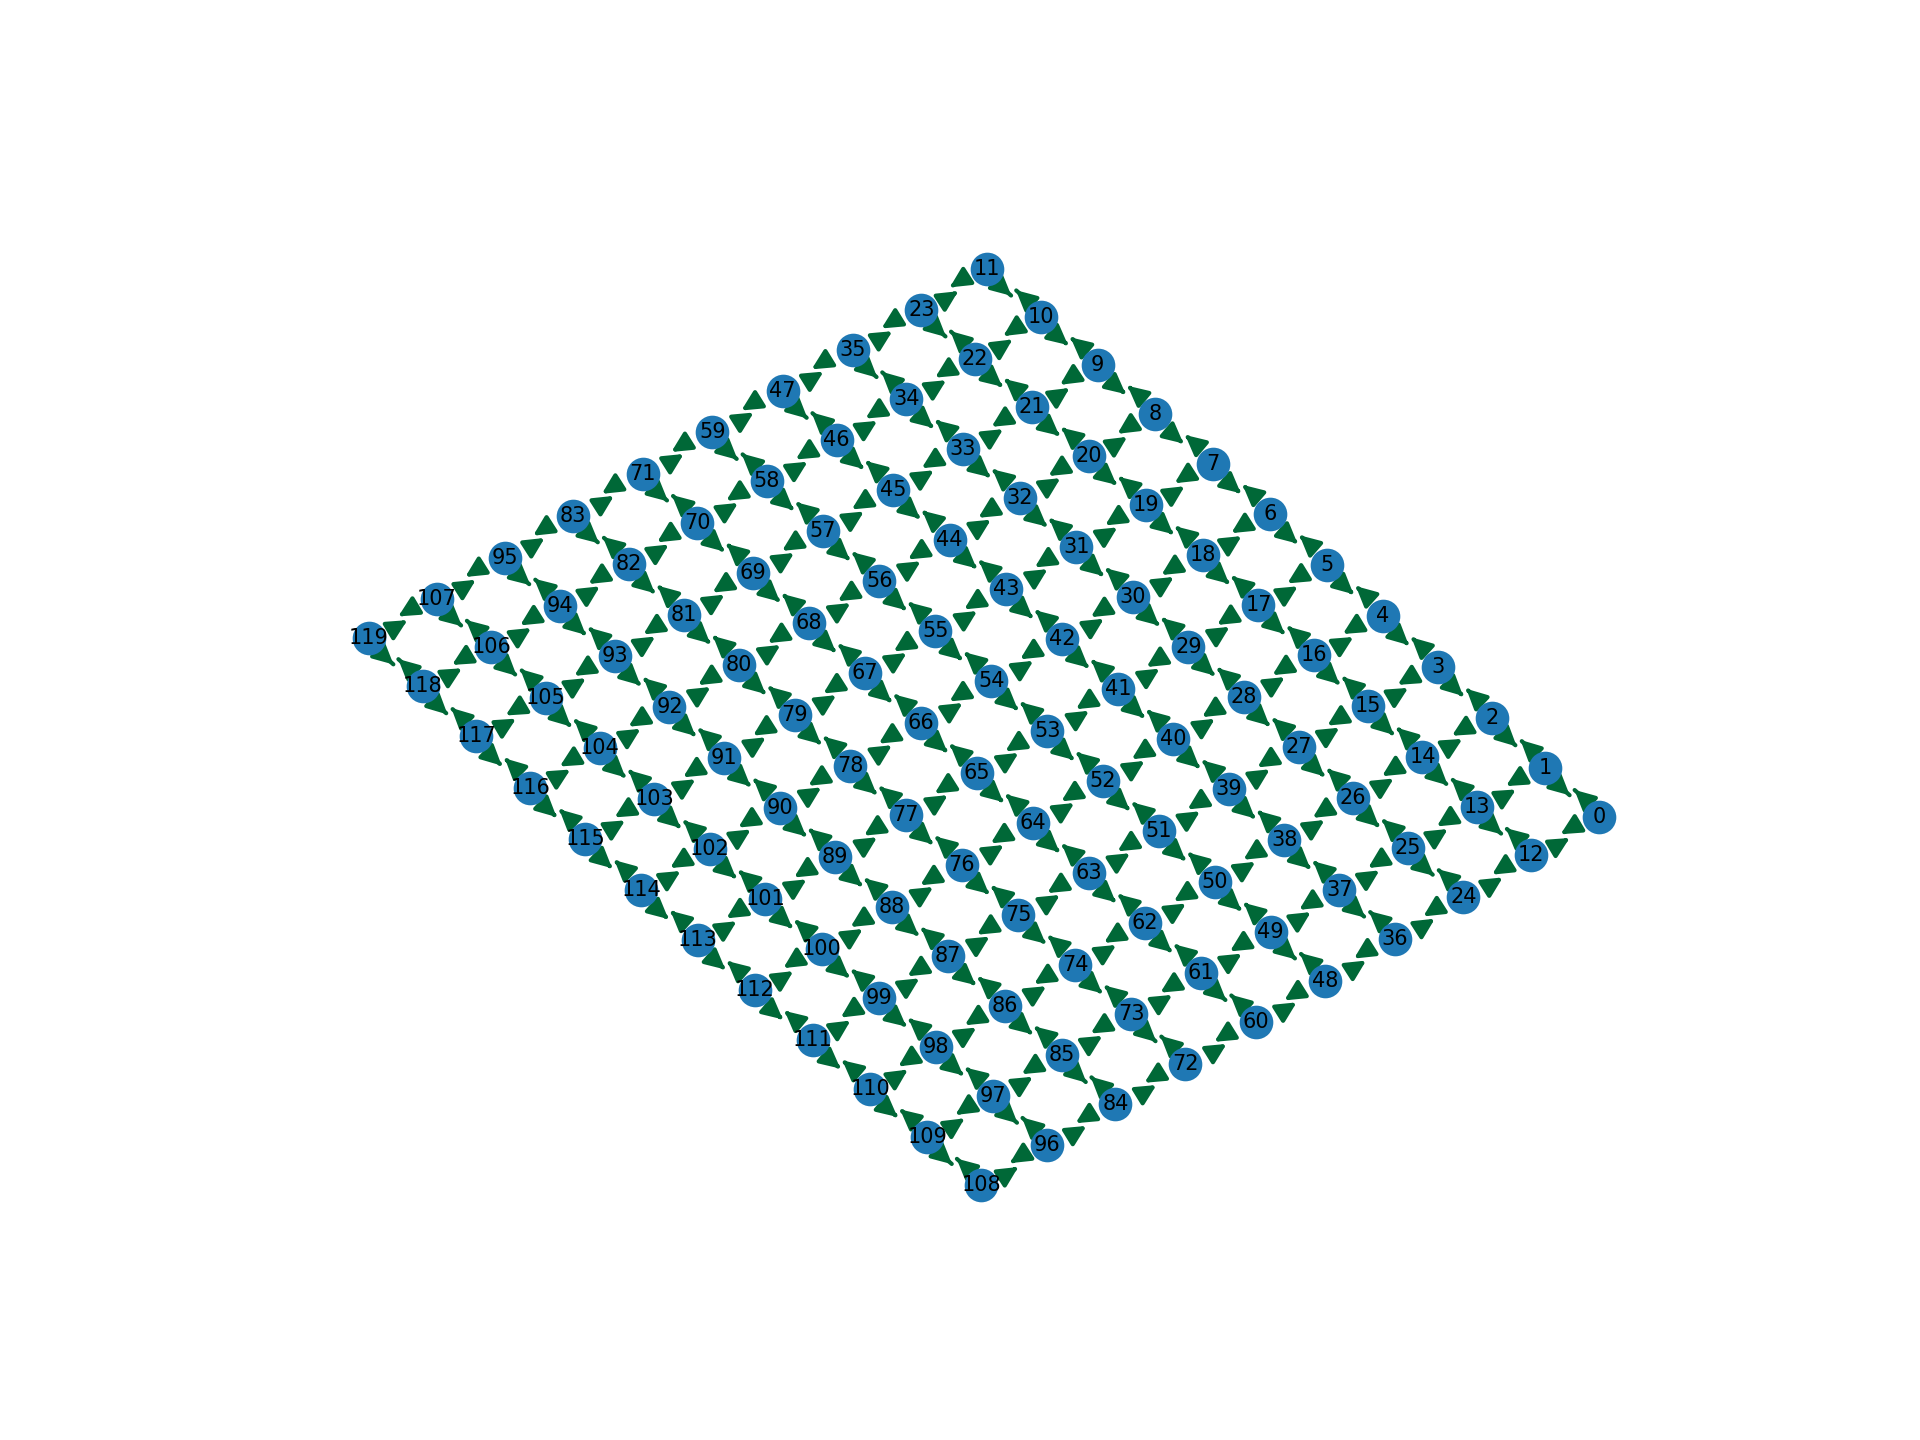
\includegraphics[scale=0.25, trim={2cm 5cm 10cm 5cm},clip]{./data/img/network.png}
    \caption[Network omogeneo]{\emph{Network omogeneo.}}
    \label{fig:network_homo}
\end{figure}
Su questo, si definiscano 16 differenti classi di veicoli, le cui sorgenti sono i nodi 1, 4, 7, 10 e le cui destinazioni sono i nodi 109, 112, 115, 118.
Risulta evidente dalla Fig. \ref{fig:network_homo} come i veicoli scorrano da un lato all'altro del reticolo.
Ogni strada ha lunghezza e velocit\`a massima fissate a 500 m e 50 km/h, rispettivamente.
Si pongano ora la lunghezza media di un veicolo pari a 8 m, la velocit\`a minima su una strada pari a $\frac{1}{4}$ della velocit\`a massima e una probabilit\`a di errore dell'8\%.

\section{Carico costante}
Si vuole, come prima cosa, sottoporre il sistema ad un carico costante: in questo modo si dovrebbe evitare la formazione di congestioni, mantenendo la capacit\`a di trasporto della rete stessa.
Il sistema viene quindi sottoposto ad un carico costante di 250 veicoli immessi ogni 60 s, fino a un tempo di 3.33 h, per un tempo totale di 4.15 h, lasciandoli liberi di uscire dalla rete una volta giunti a destinazione.
Ci si aspetta cos\`i una crescita iniziale della densit\`a media, la quale si mantiene costante fintantoch\'e nuovi veicoli vengono immessi nel sistema.
L'obiettivo \`e, infatti, mantenere complessivamente invariato il numero totale di veicoli presenti sulla rete, a meno di fluttuazioni.
\begin{figure}[H]
    \centering
    \begin{tikzpicture}
    \begin{axis}[
    grid = both,
    major grid style = {lightgray},
    minor grid style = {lightgray!25},
    width = 0.75\textwidth,
    height = 0.5\textwidth,
    ylabel near ticks,
    xlabel near ticks,
    xlabel = {Tempo (h)},
    ylabel = {Densit\`a media (veh/km)},]
    \addplot[
    mark size=0.69,
    draw=black,
    mark=o] file {./data/constant_homo/k-t.dat};
    \end{axis}
    \end{tikzpicture}
    \caption[Densit\`a media per un reticolo omogeneo con carico costante]{\emph{Densit\`a media per un reticolo omogeneo con carico costante.}}
    \label{fig:density_constant_homo}
\end{figure}
In Fig. \ref{fig:density_constant_homo} si pu\`o notare l'innalzamento iniziale, fino a circa 1.5 h, poi un regime pressoch\'e costante fino a 3.3 h, seguito da una rapida discesa.
Nell'arco temporale in cui la densit\`a \`e stabile ci si aspetta un regime di traffico completamente libero.
L'ipotesi \`e verificata in Fig. \ref{fig:nStreet_density_constant_homo} dove, graficando il numero di strade in funzione della densit\`a a 2 h, si pu\`o notare come la quasi totalit\`a di esse abbia densit\`a minima.
\begin{figure}[H]
    \centering
    \begin{tikzpicture}
    \begin{axis}[ybar interval,
    every tick label/.append style={font=\tiny},
    area style,
    width = 0.75\textwidth,
    height = 0.50\textwidth,
    xlabel = {$\frac{\rho}{\rho_{max}}$},
    ylabel = {Frequenza},]
    \addplot+[
    ybar interval,
    mark=no,
    line width = 1.25pt
    ] plot file {./data/constant_homo/7200_den.dat};
    \end{axis}
    \end{tikzpicture}
    \caption[Distribuzione delle strade non congestionate per un reticolo omogeneo.]{\emph{Distribuzione delle strade non congestionate per un reticolo omogeneo.}}
    \label{fig:nStreet_density_constant_homo}
\end{figure}
Non formandosi nessuna congestione ci si aspetta che il sistema si svuoti allo stesso modo in cui si \`e riempito.
In Fig. \ref{fig:hysteresys_constant_homo} \`e graficata la dipendenza tra i valori medi del flusso e della densit\`a.
In particolare, si nota come il grafico sia effettivamente una retta, il che implica che la curva di scarico sia sovrapposta a quella di carico.
\begin{figure}[H]
    \centering
    \begin{tikzpicture}[scale=0.75]
        \begin{axis}[
        grid = both,
        major grid style = {lightgray},
        minor grid style = {lightgray!25},
        width = 0.75\textwidth,
        height = 0.5\textwidth,
        ylabel near ticks,
        xlabel near ticks,
        xlabel = {Densità (veh/km)},
        ylabel = {Flusso (veh/h)},]
        \addplot[
        mark size=0.69,
        draw=black,
        mark=o] file {./data/constant_homo/q-k.dat};
        \end{axis}
    \end{tikzpicture}
    \caption[Diagramma flusso/densit\`a medi per un reticolo omogeneo sottoposto ad un carico costante.]{\emph{Diagramma flusso/densit\`a medi per un reticolo omogeneo sottoposto ad un carico costante.}}
    \label{fig:hysteresys_constant_homo}
\end{figure}

\section{Carico piccato}
Si inserisca ora nel sistema un totale di 25000 veicoli, suddivisi in 2500 veicoli ogni 50 s, consentendone la fuoriuscita dal reticolo solo dopo 67 min, in modo tale da lasciare al sistema tempo per giungere ad uno stato di equilibrio.
Si osserva cos\`i in Fig. \ref{fig:peaked_homo} un picco iniziale della densit\`a media (sovraccarico del sistema) e come questa rimanga stabile fino a circa 1 h da inizio simulazione, poi inizi a diminuire.
\begin{figure}[H]
    \centering
    \begin{tikzpicture}[scale=0.75]
    \begin{axis}[
    grid = both,
    major grid style = {lightgray},
    minor grid style = {lightgray!25},
    width = 0.75\textwidth,
    height = 0.5\textwidth,
    ylabel near ticks,
    xlabel near ticks,
    xlabel = {Tempo (h)},
    ylabel = {Densit\`a media (veh/km)},]
    \addplot[
    mark size=0.69,
    draw=black,
    mark=o] file {./data/peaked_homo/k-t.dat};
    \end{axis}
    \end{tikzpicture}
    \begin{tikzpicture}[scale=0.75]
        \begin{axis}[
        grid = both,
        major grid style = {lightgray},
        minor grid style = {lightgray!25},
        width = 0.75\textwidth,
        height = 0.5\textwidth,
        ylabel near ticks,
        xlabel near ticks,
        xlabel = {Tempo (h)},
        ylabel = {Flusso medio (veh/h)},]
        \addplot[
        mark size=0.69,
        draw=black,
        mark=o] file {./data/peaked_homo/q-t.dat};
        \end{axis}
        \end{tikzpicture}
    \caption[Densit\`a media per un reticolo omogeneo sovraccaricato]{\emph{Densit\`a media per un reticolo omogeneo sovraccaricato.}}
    \label{fig:peaked_homo}
\end{figure}
Una volta stabilizzato il sistema ci si aspetta che la distribuzione di veicoli nelle strade non resti omogenea nel tempo: gli agenti presenti sul sistema tenderanno ad occupare le strade costituenti i loro \emph{best path} e a lasciare vuote quelle pi\`u lontane da essi.
\begin{figure}[H]
    \centering
    \begin{tikzpicture}
    \begin{axis}[ybar interval,
    every tick label/.append style={font=\tiny},
    area style,
    width = 0.75\textwidth,
    height = 0.50\textwidth,
    xlabel = {$\frac{\rho}{\rho_{max}}$},
    ylabel = {Frequenza},]
    \addplot+[
    ybar interval,
    mark=no,
    line width = 1.25pt
    ] plot file {./data/peaked_homo/5800_den.dat};
    \end{axis}
    \end{tikzpicture}
    \caption[Distribuzione delle strade congestionate per un reticolo omogeneo.]{\emph{Distribuzione delle strade congestionate per un reticolo omogeneo.}}
    \label{fig:nStreet_density_peaked_homo}
\end{figure}
In Fig. \ref{fig:nStreet_density_peaked_homo} \`e visibile il diagramma caratteristico della congestione, in cui sono presenti, come atteso, un gran numero di strade vuote e altrettante sature.
In questo istante di tempo, pari a 1.61 h da inizio simulazione, ci si aspetta dunque che i diagrammi fondamentali siano confrontabili con quelli in Fig. \ref{fig:greenshield}: questa ipotesi \`e confermata dalla Fig. \ref{fig:DMF_peaked_homo}.
\begin{figure}[H]
    \begin{tikzpicture}[scale=0.6]
    \begin{axis}[
    grid = both,
    major grid style = {lightgray},
    minor grid style = {lightgray!25},
    width = 0.75\textwidth,
    height = 0.5\textwidth,
    ylabel near ticks,
    xlabel near ticks,
    xlabel = {Flusso (veh/h)},
    ylabel = {Velocit\`a media (km/h)},]
    \addplot[
    mark size=0.69,
    draw=black,
    only marks] file {./data/peaked_homo/5800_u-q.dat};
    \end{axis}
    \end{tikzpicture}\hfill
    \begin{tikzpicture}[scale=0.6]
        \begin{axis}[
        grid = both,
        major grid style = {lightgray},
        minor grid style = {lightgray!25},
        width = 0.75\textwidth,
        height = 0.5\textwidth,
        ylabel near ticks,
        xlabel near ticks,
        xlabel = {Densità (veh/km)},
        ylabel = {Flusso (veh/h)},]
        \addplot[
        mark size=0.69,
        draw=black,
        only marks] file {./data/peaked_homo/5800_q-k.dat};
        \end{axis}
    \end{tikzpicture}
    \centering
    \begin{tikzpicture}[scale=0.6]
    \begin{axis}[
    grid = both,
    major grid style = {lightgray},
    minor grid style = {lightgray!25},
    width = 0.75\textwidth,
    height = 0.5\textwidth,
    ylabel near ticks,
    xlabel near ticks,
    xlabel = {Densit\`a (veh/km)},
    ylabel = {Velocit\`a media (km/h)},]
    \addplot[
    mark size=0.69,
    draw=black,
    only marks] file {./data/peaked_homo/5800_u-k.dat};
    \end{axis}
    \end{tikzpicture}
    \caption[DFM per una congestione]{\emph{Diagrammi fondamentali macroscopici di una congestione in un reticolo omogeneo.}}
    \label{fig:DMF_peaked_homo}
\end{figure}
Secondo la teoria dei flussi di traffico, un sistema congestionato tende a risolvere la congestione in modo differente da come questa si \`e formata e questo fenomeno causa la formazione di un ciclo di isteresi.
Lo scarico del sistema avviene gradualmente e prevede un ritorno alla stabilit\`a lungo una traiettoria differente rispetto alla fase di carico: tale differenza \`e visibile in Fig. \ref{fig:hysteresys_peaked_homo}.
\begin{figure}[H]
    \begin{tikzpicture}[scale=0.6]
        \begin{axis}[
        grid = both,
        major grid style = {lightgray},
        minor grid style = {lightgray!25},
        width = 0.75\textwidth,
        height = 0.5\textwidth,
        ylabel near ticks,
        xlabel near ticks,
        xlabel = {Densità (veh/km)},
        ylabel = {Flusso (veh/h)},]
        \addplot[
        mark size=0.69,
        draw=black,
        mark=o] file {./data/peaked_homo/q-k.dat};
        \end{axis}
    \end{tikzpicture}\hfill
    \begin{tikzpicture}[scale=0.6]
    \begin{axis}[
    grid = both,
    major grid style = {lightgray},
    minor grid style = {lightgray!25},
    width = 0.75\textwidth,
    height = 0.5\textwidth,
    ylabel near ticks,
    xlabel near ticks,
    xlabel = {Densit\`a (veh/km)},
    ylabel = {Velocit\`a media (km/h)},]
    \addplot[
    mark size=0.69,
    draw=black,
    mark=o] file {./data/peaked_homo/u-k.dat};
    \end{axis}
    \end{tikzpicture}
    \caption[Isteresi per un reticolo omogeneo sovraccaricato]{\emph{Ciclo di isteresi per un reticolo omogeneo sovraccaricato.}}
    \label{fig:hysteresys_peaked_homo}
\end{figure}
Si pu\`o notare come sia il flusso che la densit\`a crescano fino a un punto critico nel quale si ha un calo drastico del flusso stesso dovuto all'eccessiva presenza di veicoli sulle strade.
Il sistema risulta quindi congestionato e perde la capacit\`a di trasporto.
In particolare, il massimo del flusso si ha durante la fase di carico mentre, alla fine della stessa, il sovraccarico ha gi\`a apportato modifiche al sistema, riducendone il flusso medio (cfr. Fig. \ref{fig:peaked_homo}).
Inoltre, il flusso medio del sistema tende a rimanere stabile a ridosso della congestione, a differenza della densit\`a media che risulta gi\`a in diminuzione grazie alla fuoriuscita dei primi veicoli dalla rete.

\section{Carico periodico}
Si vuole ora sottoporre il sistema ad un carico realistico, quindi variabile nell'arco di una giornata.
Per semplicit\`a si decide di trascurare il carico notturno, in quanto nella maggior parte dei casi lascia il sistema in uno stato di traffico completamente libero.
Durante il giorno, invece, si assuma una variazione periodica con diversi picchi: il primo al mattino verso le ore 9:00, seguito da una lieve discesa, il secondo verso le 13:00, un po' meno marcato, e il terzo al rientro serale, alle 17:00.
Assumendo come orario di inizio simulazione le 5:45 del mattino, si immettano veicoli uniformemente nel sistema secondo la seguente funzione:
\begin{equation}
    \Delta n(t) = A \left\lvert \sin\left(\frac{2\pi}{T}t\right) \right\rvert 
\end{equation}
con $A = 2200$ veh e $T = 32400$ s.
In questo caso, non vi \`e accumulo di veicoli: in ogni istante i veicoli che giungono a destinazione vengono eliminati.
Per rendere meno marcato il secondo picco si riduce l'ampiezza in salita di un fattore 1.125, dal primo minimo al secondo massimo.
Ci si aspetta in questo modo che, avendo la funzione tre picchi, il sistema compia tre cicli di carico e scarico.
\begin{figure}[H]
    \centering
    \begin{tikzpicture}
    \begin{axis}[
    grid = both,
    major grid style = {lightgray},
    minor grid style = {lightgray!25},
    width = 0.75\textwidth,
    height = 0.5\textwidth,
    ylabel near ticks,
    xlabel near ticks,
    xlabel = {Tempo (h)},
    ylabel = {Densit\`a media (veh/km)},]
    \addplot[
    mark size=0.69,
    draw=black,
    mark=o] file {./data/periodic_homo/k-t.dat};
    \end{axis}
    \end{tikzpicture}
    \caption[Variazione periodica della densit\`a in un reticolo omogeneo]{\emph{Variazione della densit\`a media delle strade della rete nel tempo. Si possono notare tre picchi: il primo alle 8:45, il secondo alle 13:00 e il terzo alle 17:45.}}
    \label{fig:density_time_periodic_homo}
\end{figure}
I tre picchi sono ben visibili in Fig. \ref{fig:density_time_periodic_homo}.
A ogni picco corrisponde una fase di carico/scarico, quindi, come osservato precedentemente in Fig. \ref{fig:hysteresys_peaked_homo}, ci si aspetta la presenza di tre cicli di isteresi.
\begin{figure}[H]
    \centering
    \begin{tikzpicture}
    \begin{axis}[
    grid = both,
    major grid style = {lightgray},
    minor grid style = {lightgray!25},
    width = 0.75\textwidth,
    height = 0.5\textwidth,
    ylabel near ticks,
    xlabel near ticks,
    xlabel = {Densit\`a media (veh/km)},
    ylabel = {Flusso medio (veh/h)},]
    \addplot[
    mark size=0.69,
    draw=black,
    mark=o] file {./data/periodic_homo/q-k.dat};
    \end{axis}
    \end{tikzpicture}
    \caption[Isteresi per un reticolo omogeneo caricato periodicamente]{\emph{Cicli di isteresi sul piano flusso/densit\`a per un reticolo omogeneo caricato periodicamente.}}
    \label{fig:hysteresys_periodic_homo}
\end{figure}
Come si pu\`o notare in Fig. \ref{fig:hysteresys_periodic_homo} sono effettivamente presenti tre diversi cicli di isteresi.
Si osserva, inoltre, che il secondo ciclo ha ampiezza inferiore, essendo il picco di densit\`a meno pronunciato.

\section{Tempo di percorrenza}
Un'ultima analisi effettuata riguarda il tempo di percorrenza.
Per evidenziare i comportamenti attesi rappresentati in Fig. \ref{fig:frequency_distributions} si \`e deciso di effettuare una simulazione a parte caricando progressivamente il sistema come si pu\`o notare dall'aumento della densit\`a media riportato in Fig. \ref{fig:density_travel_time}.
\begin{figure}[H]
    \centering
    \begin{tikzpicture}
    \begin{axis}[
    grid = both,
    major grid style = {lightgray},
    minor grid style = {lightgray!25},
    width = 0.75\textwidth,
    height = 0.5\textwidth,
    ylabel near ticks,
    xlabel near ticks,
    xlabel = {Tempo (h)},
    ylabel = {Densit\`a media (veh/km)},]
    \addplot[
    mark size=0.69,
    draw=black,
    mark=o] file {./data/travel_time/k-t.dat};
    \end{axis}
    \end{tikzpicture}
    \caption[Distribuzione della densit\`a media per un reticolo omogeneo caricato progressivamente]{\emph{Variazione della densit\`a media nel tempo per un reticolo omogeneo caricato progressivamente.}}
    \label{fig:density_travel_time}
\end{figure}
Dopo 50 minuti da inizio simulazione, ossia quando vi \`e ancora uno stato di traffico libero, si pu\`o notare in Fig. \ref{fig:frequency_free_flow} una distribuzione normale con media $(19.8 \pm 9.8)$ min e deviazione standard $(8.8 \pm 7.9)$ min.
\begin{figure}[H]
    \centering
    \begin{tikzpicture}
    \begin{axis}[ybar interval,
    every tick label/.append style={font=\tiny},
    area style,
    width = 0.75\textwidth,
    height = 0.5\textwidth,
    xlabel = {Tempo di percorrenza (min)},
    ylabel = {Frequenza},]
    \addplot+[
    ybar interval,
    mark=no,
    line width = 1.25pt
    ] plot file {./data/travel_time/3000_t.dat};
    \addplot[
        domain=0:100,
        smooth,
        color=red,
        line width=1.5pt
    ] {0.177299*e^(-(x-19.849)^2/(2*(8.88775)^2))};
    \end{axis}
    \end{tikzpicture}
    \caption[Distribuzione del tempo di percorrenza con traffico libero]{\emph{Distribuzione del tempo di percorrenza con traffico libero.}}
    \label{fig:frequency_free_flow}
\end{figure}
Continuando a caricare il sistema ci si aspetta che un numero sempre maggiore di individui capiti in strade trafficate, aumentando cos\`i la coda gaussiana tendente a tempi pi\`u elevati: \`e il caso riportato in Fig. \ref{fig:frequency_flow}, corrispondente a circa 90 min da inizio simulazione.
\begin{figure}[H]
    \centering
    \begin{tikzpicture}
    \begin{axis}[ybar interval,
    every tick label/.append style={font=\tiny},
    area style,
    width = 0.75\textwidth,
    height = 0.5\textwidth,
    xlabel = {Tempo di percorrenza (min)},
    ylabel = {Frequenza},]
    \addplot+[
    ybar interval,
    mark=no,
    line width = 1.25pt
    ] plot file {./data/travel_time/5200_t.dat};
    \addplot[
        domain=0:100,
        smooth,
        color=red,
        line width=1.5pt
    ] {0.113858*e^(-(x-21.9126)^2/(2*(14.7712)^2))};
    \end{axis}
    \end{tikzpicture}
    \caption[Distribuzione del tempo di percorrenza con traffico]{\emph{Distribuzione del tempo di percorrenza con traffico.}}
    \label{fig:frequency_flow}
\end{figure}
In questo caso il fit gaussiano non \`e del tutto soddisfacente. Infatti, questo riporta una media di $(22 \pm 20)$ min con una deviazione standard di $(15 \pm 18)$ min.
Con questi risultati, la probabilit\`a di avere un tempo di percorrenza maggiore di 50 min \`e dello 0.03\%, mentre i dati sperimentali riportano uno 0.04\%; tale discrepanza \`e rilevante in quanto l'ultima analisi vede un effettivo cambiamento della distribuzione.
A 190 min da inizio simulazione, infatti, il sistema risulta congestionato.
L'andamento della frequenza, riportato in Fig. \ref{fig:frequency_congested_flow}, segue un comportamento normale bimodale, in particolare la somma di due gaussiane.
\begin{figure}[H]
    \centering
    \begin{tikzpicture}
    \begin{axis}[ybar interval,
    every tick label/.append style={font=\tiny},
    area style,
    width = 0.75\textwidth,
    height = 0.5\textwidth,
    xlabel = {Tempo di percorrenza (min)},
    ylabel = {Frequenza},]
    \addplot+[
    ybar interval,
    mark=no,
    line width = 1.25pt
    ] plot file {./data/travel_time/11400_t.dat};
    \addplot[
        domain=0:100,
        smooth,
        color=red,
        line width=1.5pt
    ] {0.0551253*e^(-(x-55.86)^2/(2*(17.0398)^2))+0.0650764*e^(-(x-12.8479)^2/(2*(10.3336)^2))};
    \end{axis}
    \end{tikzpicture}
    \caption[Distribuzione del tempo di percorrenza con traffico congestionato]{\emph{Distribuzione del tempo di percorrenza con traffico congestionato.}}
    \label{fig:frequency_congested_flow}
\end{figure}
I dati restituiti dal fit di entrambe le distribuzioni sono le medie $(13 \pm 30)$ min e $(56 \pm 44)$ min con deviazioni standard pari a $(10 \pm 40)$ min e $(17 \pm 37)$ min, rispettivamente.
Complessivamente, si osserva come i due picchi mettano in evidenza le due tipologie di individui distinguibili sulla rete: quelli ``fortunati'' che continuano a impiegare una media di un quarto d'ora per percorrere il loro tratto (ritrovandosi su strade non trafficate) e quelli ``sfortunati'' che tendono a impiegare quasi un'ora a causa delle congestioni sul percorso.

\section{Discussione}
L'analisi dei diagrammi fondamentali macroscopici condotta in diverse situazioni ha evidenziato una forte dipendenza tra i valori medi di flusso, velocit\`a e densit\`a.
Inoltre, \`e emerso un legame evidente tra la formazione di congestioni e la presenza di cicli di isteresi nei diagrammi dei valori medi di flusso e densit\`a.


L'analisi del reticolo omogeneo ha evidenziato comportamenti altamente dipendenti dalla tipologia di carico a cui esso \`e stato sottoposto.
In particolare, nel caso di un carico costante, si \`e evitata completamente la creazione di congestioni, mantenendo il sistema in un costante stato di traffico completamente libero.
La mancata formazione di congestioni non ha, inoltre, permesso la formazione di cicli di isteresi, fatto osservabile negli altri due casi riportati.
Una volta sottoposto ad un carico piccato, infatti, il sistema si \`e congestionato, riducendo la propria capacit\`a di trasporto.
La riduzione della capacit\`a di trasporto \`e associabile al rapido calo del flusso medio osservabile in Fig. \ref{fig:hysteresys_peaked_homo}.
Nella stessa figura si pu\`o notare la presenza di un ciclo di isteresi dovuto alla congestione stessa, che va a chiudersi una volta permesso al sistema di svuotarsi.
Analogamente al caso precedente, nel caso di un carico periodico si osservano, in Fig. \ref{fig:hysteresys_periodic_homo}, tre cicli di isteresi differenti, ognuno corrispondente ad un diverso picco della densit\`a media (cfr Fig. \ref{fig:density_time_periodic_homo}).\\
L'analisi dei tempi di percorrenza fornisce esiti sostanzialmente coerenti con la teoria di riferimento, nonostante la grande incertezza sui dati dovuta allo scarso numero di bin in cui sono stati suddivisi gli istogrammi.
L'utilizzo di un numero pi\`u elevato di bin, tuttavia, avrebbe messo in evidenza fluttuazioni sui dati che non ne avrebbero permessa un'analisi corretta: per questo motivo i risultati ottenuti possono essere considerati qualitativamente validi.

Nonostante il modello riproduca egregiamente numerose caratteristiche delle congestioni di traffico risulta sostanzialmente incompleto.
Manca, ad esempio, la possibilit\`a di ricalcolare i \emph{best path} in base alle condizioni istantanee di traffico e l'implementazione di alcune caratteristiche tipiche degli OVM (\emph{Optimal Velocity Model}) come la dipendenza della velocit\`a e della distanza di un veicolo in base a quella del veicolo che lo precede e l'accelerazione dei veicoli stessi.
Ulteriori studi potrebbero essere svolti per verificare come una o pi\`u queste revisioni impattino sui DFM.

\appendix

\newpage
\thispagestyle{empty}
\mbox{}

\chapter{Esempi di matrici Laplaciane}
\label{appendix:laplacian}
Si vuole qui dare un esempio di come una matrice Laplaciana venga realmente costruita e una breve analisi degli autovalori.
Si consideri come primo esempio il network completamente connesso rappresentato in Fig. \ref{fig:network_connesso}.
\begin{figure}[H]
    \centering
    \begin{tikzpicture}[>=latex,every node/.style={draw,circle,minimum width={3em},node distance=6em}]
    \node (2) {2};
    \node [above left of=2] (0) {0}; 
    \node [above right of=2] (1) {1};
    \node [below of=2] (3) {3};  
    \draw [<->] (2) -- (0);
    \draw [<->] (2) -- (1);
    \draw [<->] (0) -- (1);
    \draw [<->] (2) -- (3);
    \end{tikzpicture}
    \caption[Grafo di un network connesso]{\emph{Esempio network connesso.}}
    \label{fig:network_connesso}
\end{figure}
Questo \`e descritto dalla matrice di adiacenza:
\begin{equation}
    \mathcal{A}=\left(
    \begin{matrix}
        0 & 1 & 1 & 0\\
        1 & 0 & 1 & 0\\
        1 & 1 & 0 & 1\\
        0 & 0 & 1 & 0
    \end{matrix}\right)
\end{equation}
La matrice Laplaciana costruita dalla definizione risulta
\begin{equation}
    \mathcal{L}=\left(
    \begin{matrix}
        2 & -1 & -1 & 0\\
        -1 & 2 & -1 & 0\\
        -1 & -1 & 3 & -1\\
        0 & 0 & -1 & 1
    \end{matrix}\right)
\end{equation}
la quale possiede autovalori 0, 1, 3, 4.
In particolare, si nota la presenza dell'autovalore nullo, come previsto teoricamente.\\
Si esegua ora la stessa analisi per un network disconnesso, come quello in Fig. \ref{fig:network_sconnesso}.
\begin{figure}[H]
    \centering
    \begin{tikzpicture}[>=latex,every node/.style={draw,circle,minimum width={3em},node distance=6em}]
    \node (0) {0};
    \node [above right of=0] (1) {1}; 
    \node [below right of=1] (2) {2};
    \node [right of=2] (3) {3};
    \node [below right of=3] (4) {4};
    \node [above right of=4] (5) {5};
    \draw [<->] (0) -- (1);
    \draw [<->] (1) -- (2);
    \draw [<->] (3) -- (4);
    \draw [<->] (4) -- (5);
    \draw [<->] (3) -- (5);
    \end{tikzpicture}
    \caption[Grafo di un network sconnesso]{\emph{Esempio network sconnesso.}}
    \label{fig:network_sconnesso}
\end{figure}
La matrice di adiacenza \`e
\begin{equation}
    \mathcal{A}=\left(
    \begin{matrix}
        0 & 1 & 0 & 0 & 0 & 0\\
        1 & 0 & 1 & 0 & 0 & 0\\
        0 & 1 & 0 & 0 & 0 & 0\\
        0 & 0 & 0 & 0 & 1 & 1\\
        0 & 0 & 0 & 1 & 0 & 1\\
        0 & 0 & 0 & 1 & 1 & 0\\
    \end{matrix}\right)
\end{equation}
La matrice Laplaciana in questo caso diviene
\begin{equation}
    \mathcal{L}=\left(
    \begin{matrix}
        1 & -1 & 0 & 0 & 0 & 0\\
        -1 & 1 & -1 & 0 & 0 & 0\\
        0 & -1 & 1 & 0 & 0 & 0\\
        0 & 0 & 0 & 2 & -1 & -1\\
        0 & 0 & 0 & -1 & 2 & -1\\
        0 & 0 & 0 & -1 & -1 & 2\\
    \end{matrix}\right)
\end{equation}
ed ha autovalori 0, 0, 1, 2, 3, 3.
Anche in questo caso vi sono due autovalori nulli, essendo il network sconnesso, come previsto dalla teoria.
\chapter{Visualizzazione del sistema}
\label{appendix:visual}
Tramite uno script Python \`e stato possibile visualizzare determinati stati del sistema.
Per visualizzare al meglio la rete si \`e scelto di riportare i grafi relativi allo studio dei tempi di percorrenza.
Nel regime di traffico libero, cfr. Fig. \ref{fig:frequency_free_flow}, ci si aspetta che la quasi totalit\`a delle strade sia vuota.
\begin{figure}
    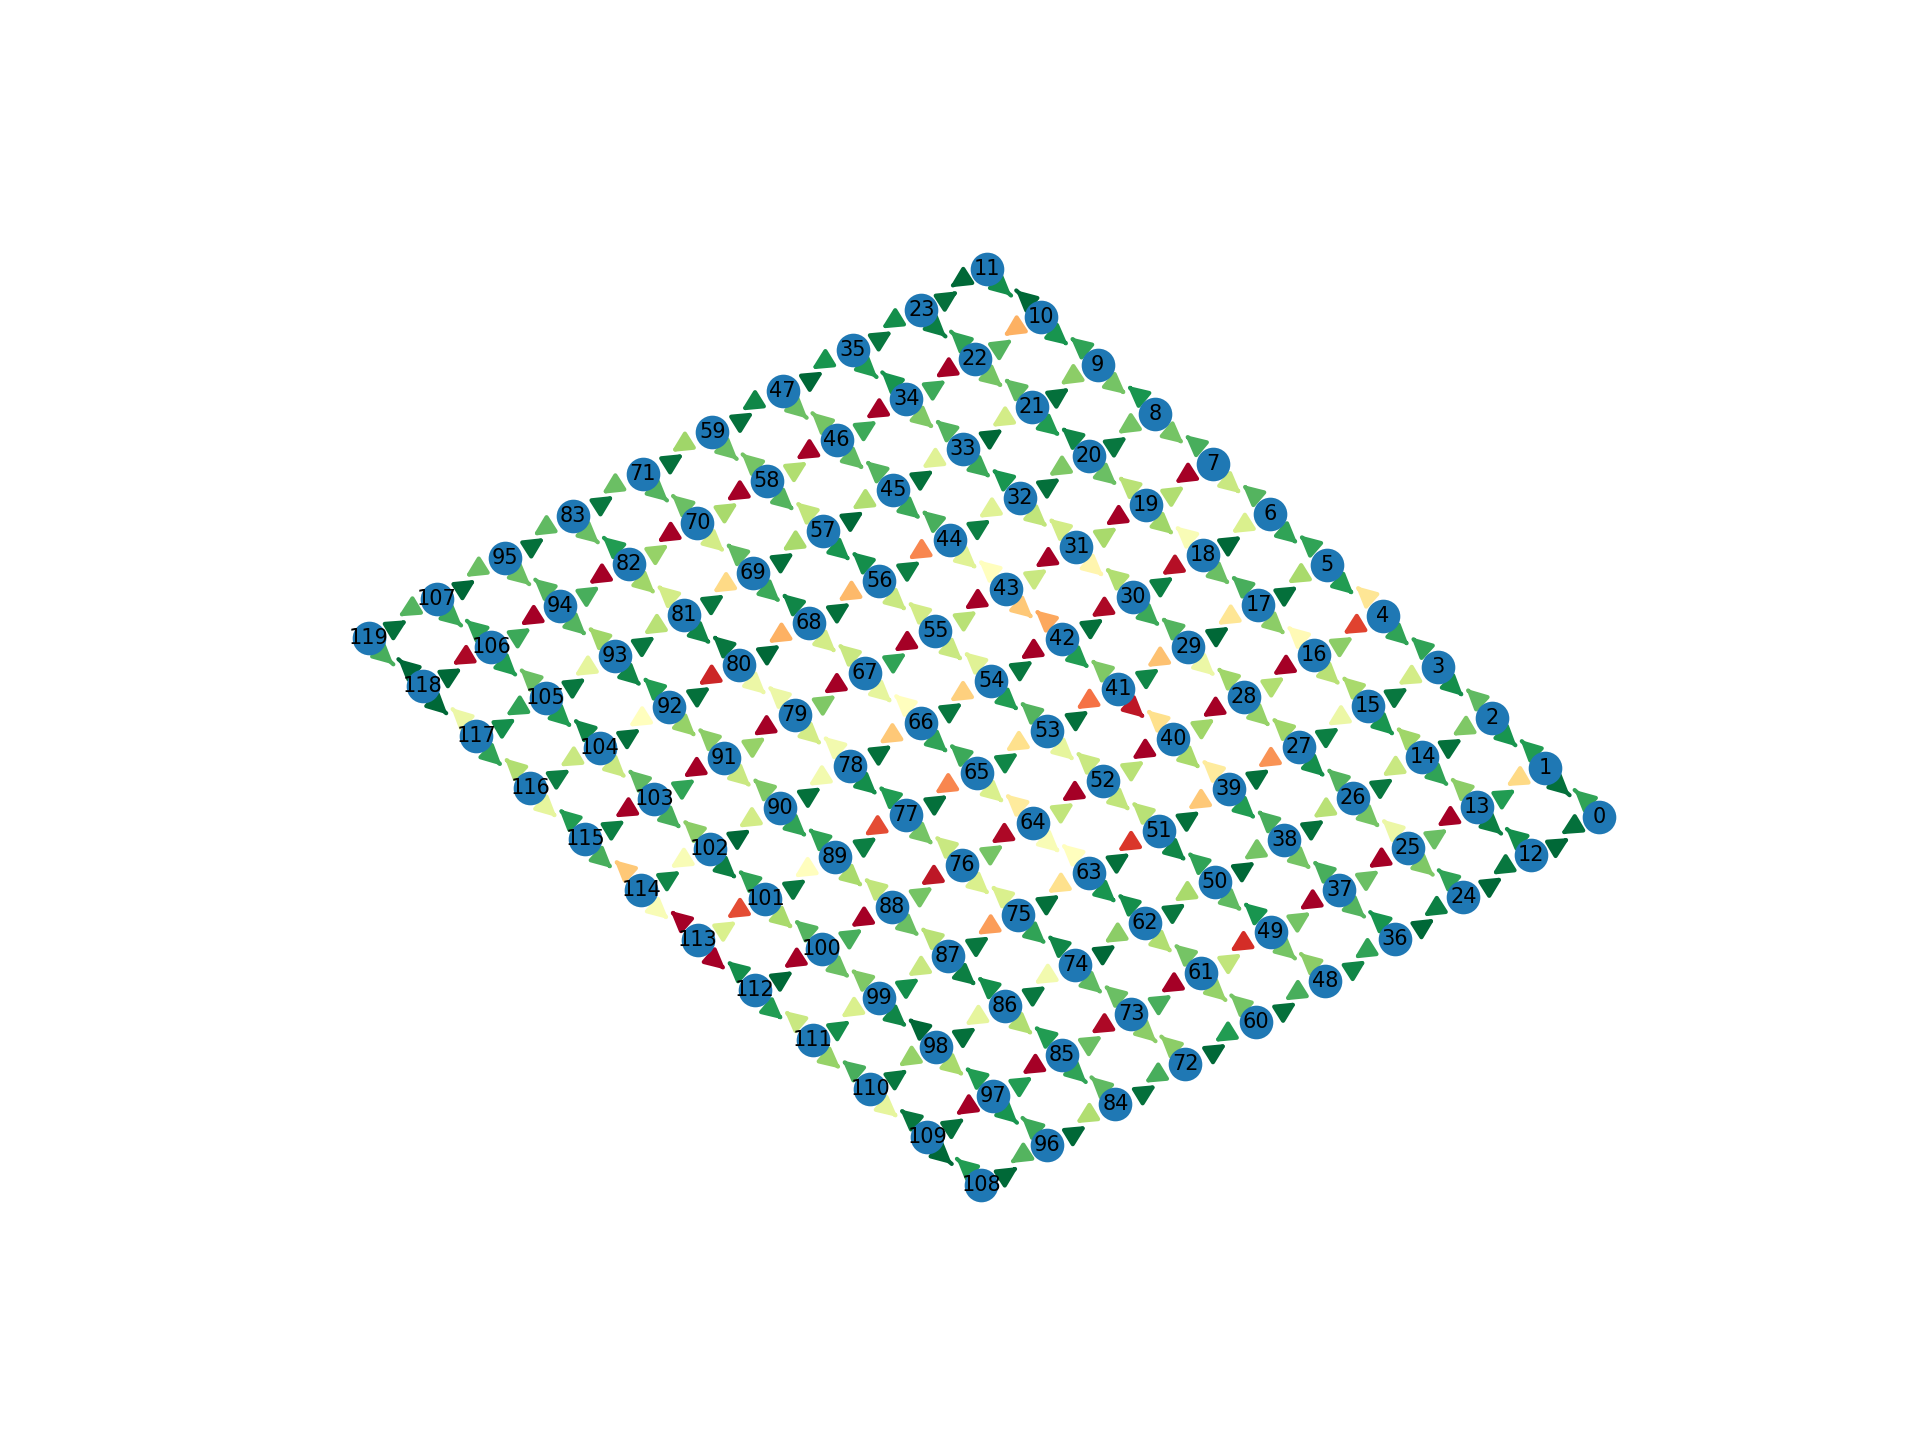
\includegraphics[scale=0.25, trim={2cm 5cm 10cm 5cm},clip]{./data/img/free_flow.png}
    \caption[Visualizzazione della rete non congestionata.]{\emph{Visualizzazione della rete non congestionata.}}
    \label{fig:visual_free}
\end{figure}
In Fig. \ref{fig:visual_free} si nota come gli unici percorsi congestionati, di colore rosso, siano le vie dirette dai nodi sorgenti alle destinazioni.
\begin{figure}
    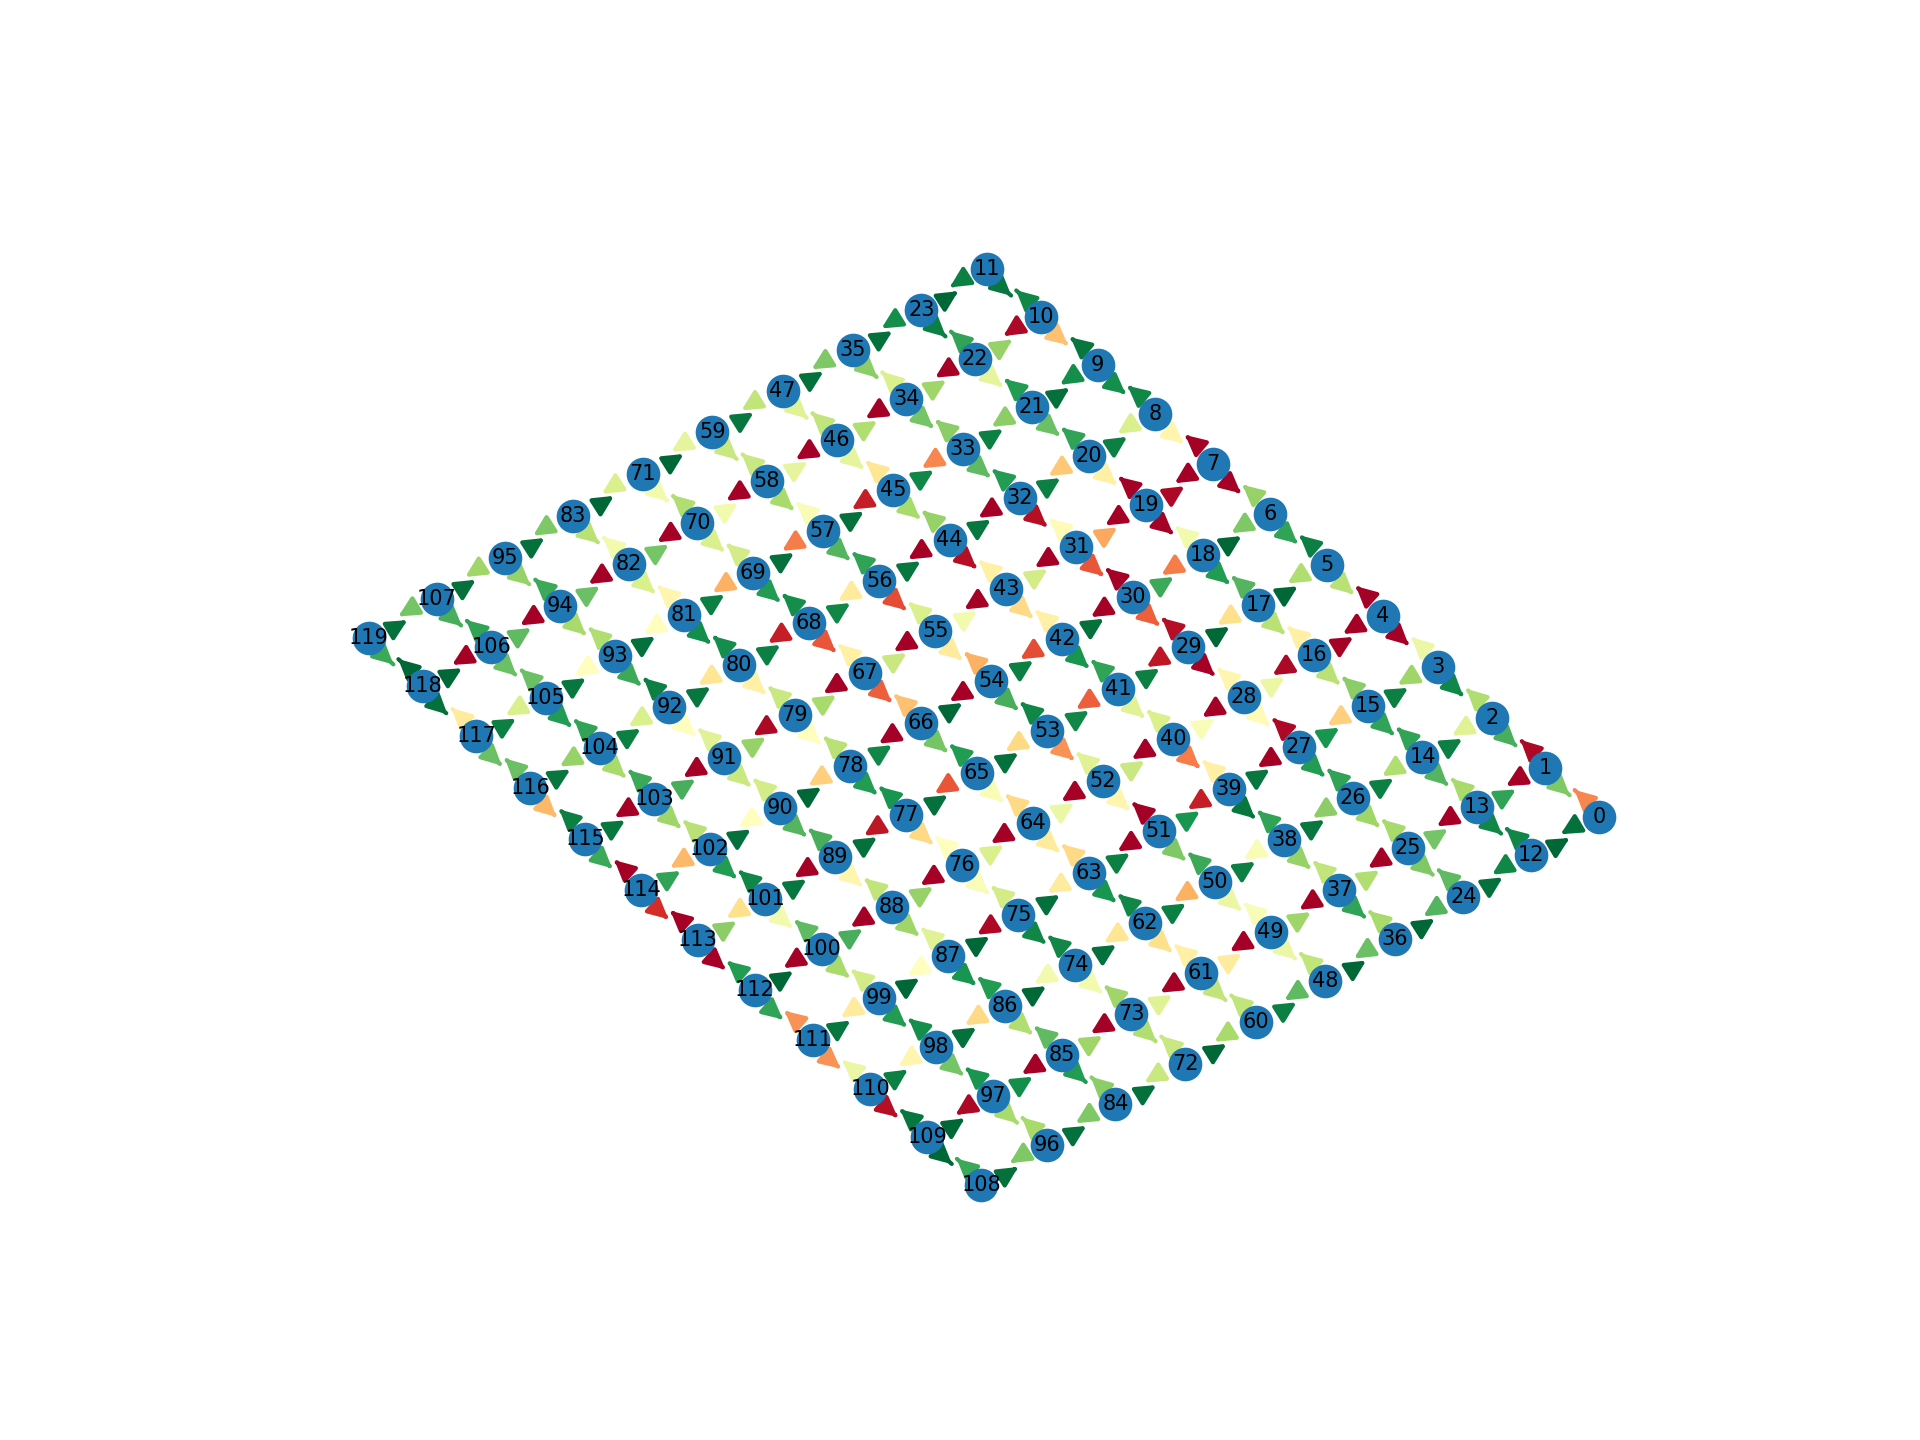
\includegraphics[scale=0.25, trim={2cm 5cm 10cm 5cm},clip]{./data/img/flow.png}
    \caption[Visualizzazione della rete mediamente congestionata.]{\emph{Visualizzazione della rete mediamente congestionata.}}
    \label{fig:visual_medium}
\end{figure}
In Fig. \ref{fig:visual_medium}, invece, il sistema comincia a entrare in congestione (cfr Fig. \ref{fig:frequency_flow}): si osservano cambiamenti nella densit\`a di veicoli sulle strade ortogonali ai percorsi diretti.
\begin{figure}
    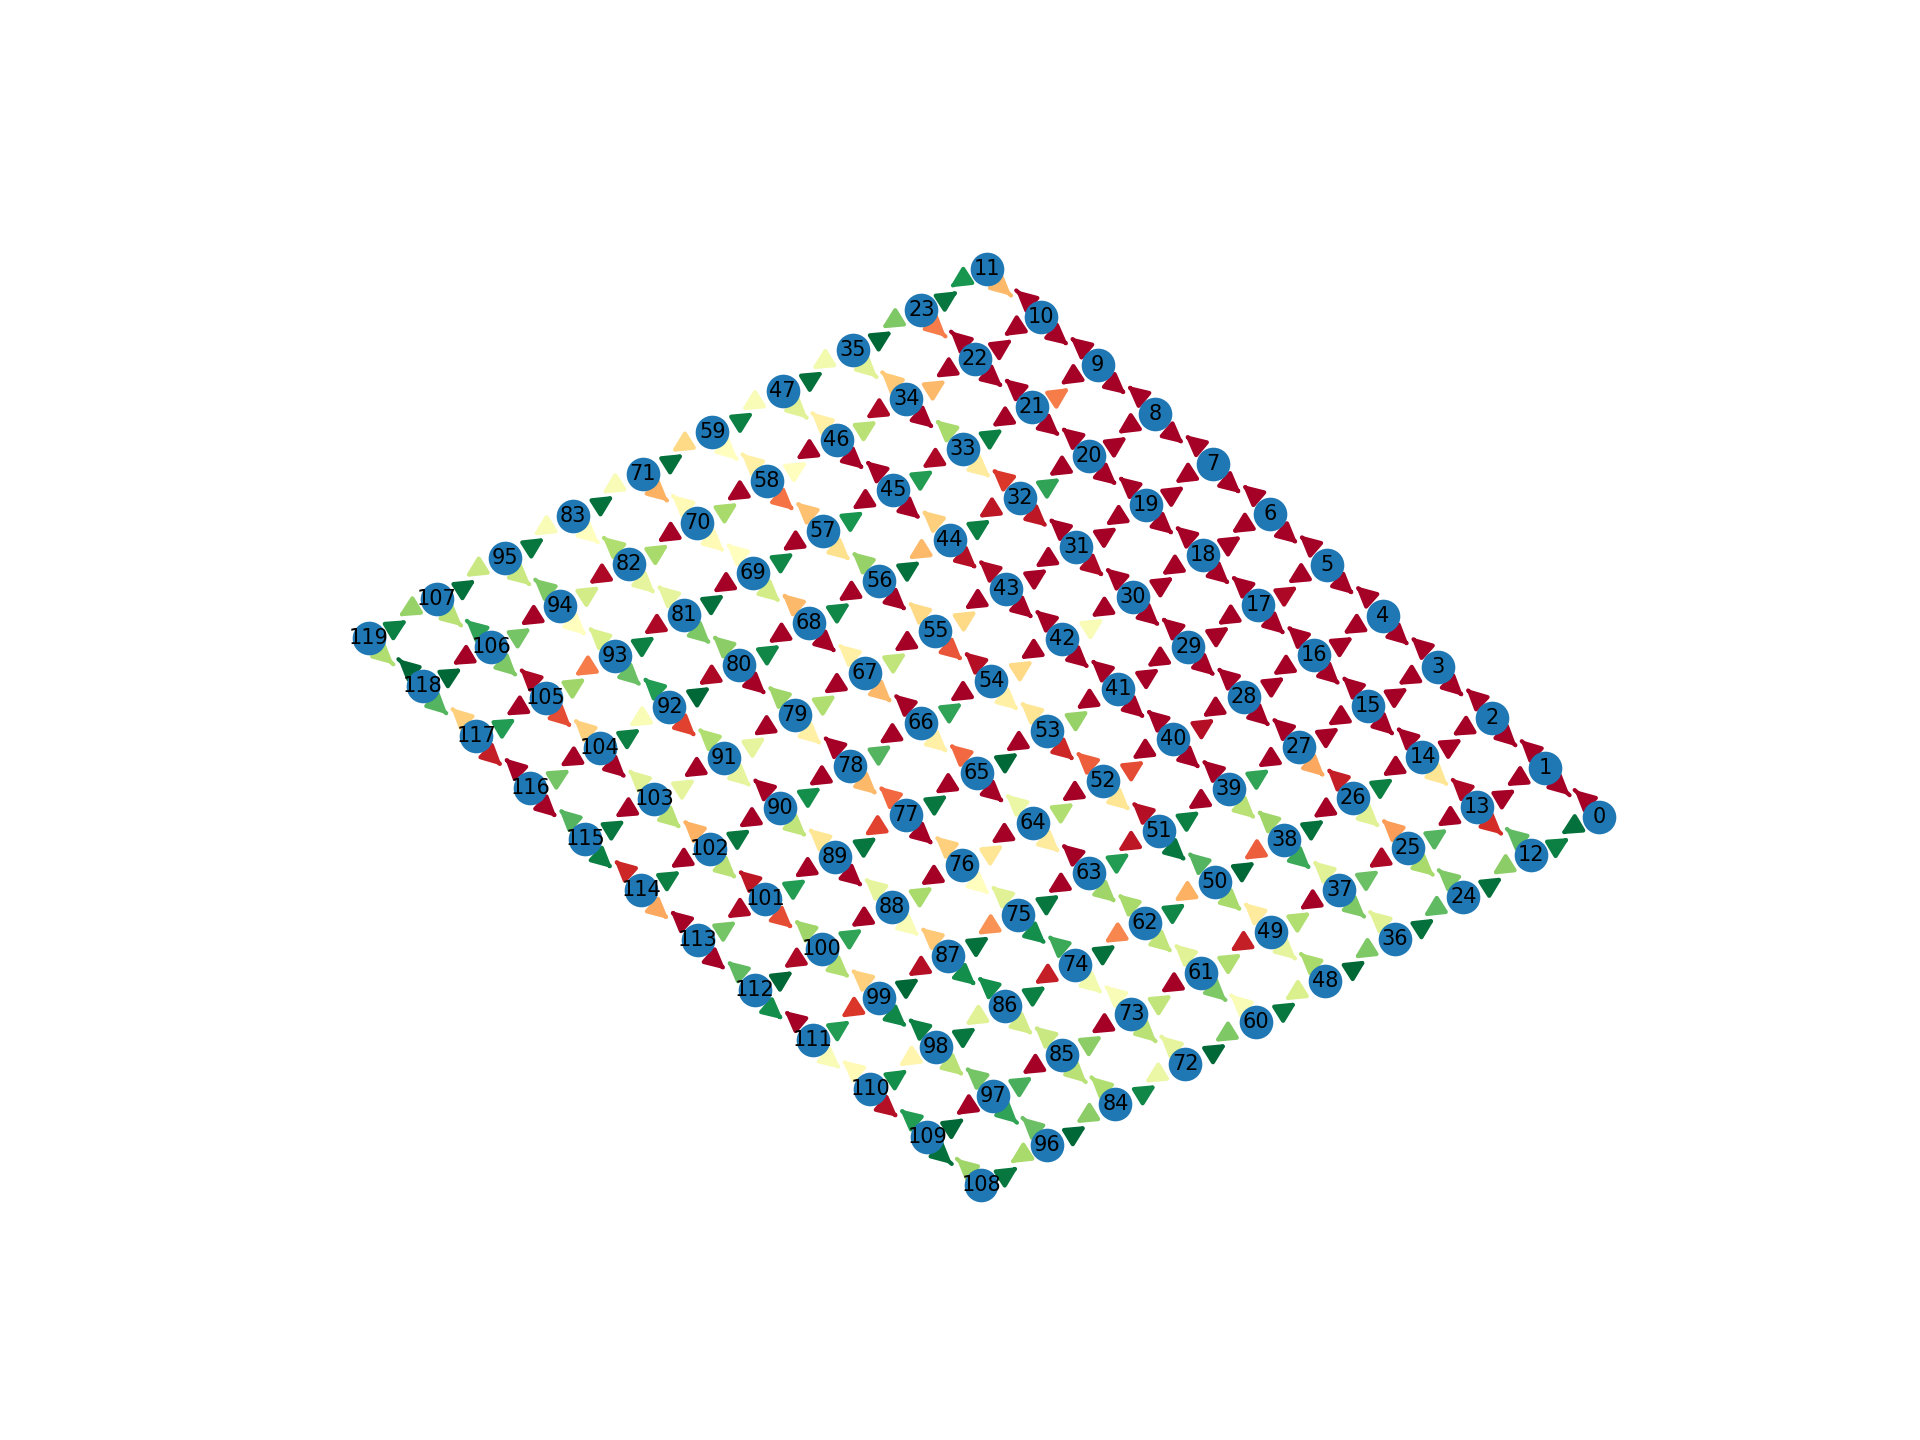
\includegraphics[scale=0.25, trim={2cm 5cm 10cm 5cm},clip]{./data/img/congested_flow.png}
    \caption[Visualizzazione della rete congestionata.]{\emph{Visualizzazione della rete congestionata.}}
    \label{fig:visual_congested}
\end{figure}
Infine, in Fig. \ref{fig:visual_congested} il sistema \`e congestionato e si ha una densit\`a di veicoli decisamente elevata in prossimit\`a dei nodi sorgente, cfr Fig. \ref{fig:frequency_congested_flow}.

\newpage
\thispagestyle{empty}
\mbox{}

\printbibliography
\end{document}
